%% Run LaTeX on this file several times to get Table of Contents,
%% cross-references, and citations.

\documentclass[11pt]{book}
\usepackage{gvv-book}
\usepackage{gvv}
\usepackage{hyperref}
\usepackage{tikz}
\usetikzlibrary{positioning}
\usetikzlibrary{arrows.meta} % for arrow tips
\usepackage{textcomp} % for \perthousand
\usepackage{siunitx} % for \micro
\usepackage{pgfplots}
%\usepackage{Wiley-AuthoringTemplate}
\usepackage[sectionbib,authoryear]{natbib}% for name-date citation comment the below line
%\usepackage[sectionbib,numbers]{natbib}% for numbered citation comment the above line

%%********************************************************************%%
%%       How many levels of section head would you like numbered?     %%
%% 0= no section numbers, 1= section, 2= subsection, 3= subsubsection %%
\setcounter{secnumdepth}{3}
%%********************************************************************%%
%%**********************************************************************%%
%%     How many levels of section head would you like to appear in the  %%
%%				Table of Contents?			%%
%% 0= chapter, 1= section, 2= subsection, 3= subsubsection titles.	%%
\setcounter{tocdepth}{2}
%%**********************************************************************%%

%\includeonly{ch01}
\makeindex

\begin{document}

\frontmatter
%%%%%%%%%%%%%%%%%%%%%%%%%%%%%%%%%%%%%%%%%%%%%%%%%%%%%%%%%%%%%%%%
%% Title Pages
%% Wiley will provide title and copyright page, but you can make
%% your own titlepages if you'd like anyway
%% Setting up title pages, type in the appropriate names here:

\booktitle{Signal Processing}

\subtitle{Through GATE}

\AuAff{EE1205-TA Group \\ \vspace{12pt} \small{Author: Sayyam Palrecha}}
%\lfill{Sayyam Palrecha}
%% \\ will start a new line.
%% You may add \affil{} for affiliation, ie,
%\authors{Robert M. Groves\\
%\affil{Universitat de les Illes Balears}
%Floyd J. Fowler, Jr.\\
%\affil{University of New Mexico}
%}

%% Print Half Title and Title Page:
%\halftitlepage
\titlepage

%%%%%%%%%%%%%%%%%%%%%%%%%%%%%%%%%%%%%%%%%%%%%%%%%%%%%%%%%%%%%%%%
%% Copyright Page

\begin{copyrightpage}{2024}
%Title, etc
\end{copyrightpage}

% Note, you must use \ to start indented lines, ie,
% 
% \begin{copyrightpage}{2004}
% Survey Methodology / Robert M. Groves . . . [et al.].
% \       p. cm.---(Wiley series in survey methodology)
% \    ``Wiley-Interscience."
% \    Includes bibliographical references and index.
% \    ISBN 0-471-48348-6 (pbk.)
% \    1. Surveys---Methodology.  2. Social 
% \  sciences---Research---Statistical methods.  I. Groves, Robert M.  II. %
% Series.\\

% HA31.2.S873 2004
% 001.4'33---dc22                                             2004044064
% \end{copyrightpage}

%%%%%%%%%%%%%%%%%%%%%%%%%%%%%%%%%%%%%%%%%%%%%%%%%%%%%%%%%%%%%%%%
%% Only Dedication (optional) 

%\dedication{To my parents}

\tableofcontents

%\listoffigures %optional
%\listoftables  %optional

%% or Contributor Page for edited books
%% before \tableofcontents

%%%%%%%%%%%%%%%%%%%%%%%%%%%%%%%%%%%%%%%%%%%%%%%%%%%%%%%%%%%%%%%%
%  Contributors Page for Edited Book
%%%%%%%%%%%%%%%%%%%%%%%%%%%%%%%%%%%%%%%%%%%%%%%%%%%%%%%%%%%%%%%%

% If your book has chapters written by different authors,
% you'll need a Contributors page.

% Use \begin{contributors}...\end{contributors} and
% then enter each author with the \name{} command, followed
% by the affiliation information.

% \begin{contributors}
% \name{Masayki Abe,} Fujitsu Laboratories Ltd., Fujitsu Limited, Atsugi, Japan
%
% \name{L. A. Akers,} Center for Solid State Electronics Research, Arizona State University, Tempe, Arizona
%
% \name{G. H. Bernstein,} Department of Electrical and Computer Engineering, University of Notre Dame, Notre Dame, South Bend, Indiana; formerly of
% Center for Solid State Electronics Research, Arizona
% State University, Tempe, Arizona 
% \end{contributors}

%%%%%%%%%%%%%%%%%%%%%%%%%%%%%%%%%%%%%%%%%%%%%%%%%%%%%%%%%%%%%%%%
% Optional Foreword:

%\begin{foreword}
%\lipsum[1-2]
%\end{foreword}

%%%%%%%%%%%%%%%%%%%%%%%%%%%%%%%%%%%%%%%%%%%%%%%%%%%%%%%%%%%%%%%%
% Optional Preface:

%\begin{preface}
%\lipsum[1-1]
%\prefaceauthor{}
%\where{place\\
% date}
%\end{preface}

% ie,
% \begin{preface}
% This is an example preface.
% \prefaceauthor{R. K. Watts}
% \where{Durham, North Carolina\\
% September, 2004}

%%%%%%%%%%%%%%%%%%%%%%%%%%%%%%%%%%%%%%%%%%%%%%%%%%%%%%%%%%%%%%%%
% Optional Acknowledgments:

%\acknowledgments
%\lipsum[1-2]
%\authorinitials{I. R. S.}  

%%%%%%%%%%%%%%%%%%%%%%%%%%%%%%%%
%% Glossary Type of Environment:

% \begin{glossary}
% \term{<term>}{<description>}
% \end{glossary}

%%%%%%%%%%%%%%%%%%%%%%%%%%%%%%%%
%\begin{acronyms}
%\acro{ASTA}{Arrivals See Time Averages}
%\acro{BHCA}{Busy Hour Call Attempts}
%\acro{BR}{Bandwidth Reservation}
%\acro{b.u.}{bandwidth unit(s)}
%\acro{CAC}{Call / Connection Admission Control}
%\acro{CBP}{Call Blocking Probability(-ies)}
%\acro{CCS}{Centum Call Seconds}
%\acro{CDTM}{Connection Dependent Threshold Model}
%\acro{CS}{Complete Sharing}
%\acro{DiffServ}{Differentiated Services}
%\acro{EMLM}{Erlang Multirate Loss Model}
%\acro{erl}{The Erlang unit of traffic-load}
%\acro{FIFO}{First in - First out}
%\acro{GB}{Global balance}
%\acro{GoS}{Grade of Service}
%\acro{ICT}{Information and Communication Technology}
%\acro{IntServ}{Integrated Services}
%\acro{IP}{Internet Protocol}
%\acro{ITU-T}{International Telecommunication Unit -- Standardization sector}
%\acro{LB}{Local balance}
%\acro{LHS}{Left hand side}
%\acro{LIFO}{Last in - First out}
%\acro{MMPP}{Markov Modulated Poisson Process}
%\acro{MPLS}{Multiple Protocol Labeling Switching}
%\acro{MRM}{Multi-Retry Model}
%\acro{MTM}{Multi-Threshold Model}
%\acro{PASTA}{Poisson Arrivals See Time Averages}
%\acro{PDF}{Probability Distribution Function}
%\acro{pdf}{probability density function}
%\acro{PFS}{Product Form Solution}
%\acro{QoS}{Quality of Service}
%\acro{r.v.}{random variable(s)}
%\acro{RED}{random early detection}
%\acro{RHS}{Right hand side}
%\acro{RLA}{Reduced Load Approximation}
%\acro{SIRO}{service in random order}
%\acro{SRM}{Single-Retry Model}
%\acro{STM}{Single-Threshold Model}
%\acro{TCP}{Transport Control Protocol}
%\acro{TH}{Threshold(s)}
%\acro{UDP}{User Datagram Protocol}
%\end{acronyms}

\setcounter{page}{1}

\begin{introduction}
This book provides solutions to signal processing problems in GATE.

\end{introduction}

\mainmatter
\chapter{Harmonics}
\section{2021}
\begin{enumerate}[label=\thechapter.\arabic*,ref=\thechapter.\theenumi]
\item 
\solution
\input{}
\pagebreak
\end{enumerate}

\section{2021}
\chapter{Filters}
\section{2021}
\begin{enumerate}[label=\thechapter.\arabic*,ref=\thechapter.\theenumi]
\item 
\solution
\input{}
\pagebreak
\end{enumerate}

\section{2021}
\chapter{ Z-transform}
\section{2021}
\begin{enumerate}[label=\thechapter.\arabic*,ref=\thechapter.\theenumi]
\item The causal signal with Z transform $z^2(z - a)^{-2}$ is ($u(n)$ is unit step signal)
\begin{enumerate}
    \item $a^{2n}u(n)$
    \item $(n + 1)a^nu(n)$
    \item $n^{-1}a^nu(n)$
    \item $n^2a^nu(n)$
\end{enumerate}

\hfill(GATE 31 EE 2021) 

\solution
 \iffalse
\let\negmedspace\undefined
\let\negthickspace\undefined
\documentclass[journal,12pt,twocolumn]{IEEEtran}
\usepackage{cite}
\usepackage{amsmath,amssymb,amsfonts,amsthm}
\usepackage{algorithmic}
\usepackage{graphicx}
\usepackage{textcomp}
\usepackage{xcolor}
\usepackage{txfonts}
\usepackage{listings}
\usepackage{enumitem}
\usepackage{mathtools}
\usepackage{gensymb}
\usepackage{comment}
\usepackage[breaklinks=true]{hyperref}
\usepackage{tkz-euclide} 
\usepackage{tikz}
% \usetikzlibrary{positioning, arrows.meta}
\usepackage{listings}
\usepackage{gvv} 
\usepackage{caption}
\def\inputGnumericTable{}                   

%\usepackage[latin1]{inputenc}                                
\usepackage{color}                                            
\usepackage{array}                                            
\usepackage{longtable}                                       
\usepackage{calc}                                             
\usepackage{multirow}                                         
\usepackage{hhline}                                           
\usepackage{ifthen}                                           
\usepackage{lscape}
\usepackage{tikz}
\newtheorem{theorem}{Theorem}[section]
\newtheorem{problem}{Problem}
\newtheorem{proposition}{Proposition}[section]
\newtheorem{lemma}{Lemma}[section]
\newtheorem{corollary}[theorem]{Corollary}
\newtheorem{example}{Example}[section]
\newtheorem{definition}[problem]{Definition}
\newcommand{\BEQA}{\begin{eqnarray}}
\newcommand{\EEQA}{\end{eqnarray}}
\newcommand{\define}{\stackrel{\triangle}{=}}
\theoremstyle{remark}
\newtheorem{rem}{Remark}

\begin{document}

\bibliographystyle{IEEEtran}
\vspace{3cm}

\title{GATE: EE - 31.2021}
\author{EE23BTECH11013 - Avyaaz$^{*}$% <-this % stops a space 
}
\maketitle
\newpage
\bigskip

\renewcommand{\thefigure}{\arabic{figure}}
\renewcommand{\thetable}{\arabic{table}}

\large\textbf{\textsl{Question:}}
The causal signal with Z transform $z^2(z - a)^{-2}$ is ($u(n)$ is unit step signal)
\begin{enumerate}
    \item $a^{2n}u(n)$
    \item $(n + 1)a^nu(n)$
    \item $n^{-1}a^nu(n)$
    \item $n^2a^nu(n)$
\end{enumerate}

\hfill(GATE EE 2021) \\
\solution
\fi
% \begin{table}[htbp]
%     \centering
%      \begin{tabular}{|c|c|c|}
\hline
    Parameter & Description & Value\\
    \hline
    $P(s)$ & Plant Transfer Function & $\frac{0.001}{s\brak{\frac{s}{0.5}+1}\brak{\frac{s}{100}+1}}$\\
    \hline
    $C(s)$ & Lag Compensator  & $\frac{100\brak{\frac{s}{10}+1}}{\frac{s}{0.1}+1}$\\
    \hline
    $T(s)$ & Loop gain  & $P(s) C(s)$ \\
    \hline
    $\omega$ & Angular Frequency & 3rad/s \\
    \hline
\end{tabular}

%     \caption{}
%     \label{tab:my_label.41.IN.2022}
% \end{table}

% \begin{figure}[!htbp]
%     \resizebox{0.501\textwidth}{!}{\documentclass{standalone}
\usepackage{tikz}
\usepackage{graphicx} % For rotatebox
\usetikzlibrary{circuits.ee.IEC}

\begin{document}
\begin{tikzpicture}[circuit ee IEC, scale=0.8, transform shape]

% Define components
\def\kone{2} % Capacitance 1/k1
\def\ktwo{3} % Capacitance 1/k2
\def\lone{1.5} % Inductance L1

% Draw parallel combination
\draw[fill=gray!30] (0,0) to [capacitor={info={$\frac{1}{k_1}$}}] ++(1.5,0) coordinate (C1)
            to [inductor={info'={$L_1$}, swap}] ++(1.5,0) coordinate (L1);

% Add parallel combination with L2 and 1/k2
\draw[fill=gray!30] (C1) ++(1.5,0) to [capacitor={info={\rotatebox{90}{$\frac{1}{k_2}$}}}] ++(0,-1.5) coordinate (C2);
\draw[fill=gray!30] (C2) ++(2,1.5) to [inductor={info'={\rotatebox{90}{$L_2$}}, swap}] ++(0,-1.5) coordinate (L2);

% Join L1 and L2 with a solid line
\draw (0,-1.5) -- (L2);
\draw (0,0) -- (0,-1.5);
\draw (3,0) --(5,0);

% Add pointer and label for i1
\draw[postaction={decorate,decoration={markings,mark=at position 0.5 with {\arrow{>}}}}] (0,0) -- node[above] {\(i_1\)} (0.5,0);

% Add pointer and label for i2
\draw[postaction={decorate,decoration={markings,mark=at position 0.5 with {\arrow{>}}}}] (3,0) -- node[above] {\(i_2\)} (3.5,0);

\end{tikzpicture}
\end{document}

}
%     \caption{Block Diagram of System}
%     \label{fig:gate_IN_Q41_blockdiagram}
% \end{figure}


Z-transform of a causal signal is, 
\begin{align}
    X(z) = z^2(z - a)^{-2} = \frac{1}{(1 - az^{-1})^2};|z| > |a|\label{eq:given.EE.31.2021}
\end{align}
The Z transform pair for $a^nu(n)$ signal is given by :
\begin{align}
    a^nu(n) \longleftrightarrow \frac{1}{1 - az^{-1}}
\end{align}
Using differentiation in z-domain property:
\begin{align}
    na^nu(n) &\longleftrightarrow -z\frac{d}{dz}\left(\frac{1}{1 - az^{-1}}\right) \\
     \implies    na^nu(n) &\longleftrightarrow \frac{az^{-1}}{(1 - az^{-1})^2}
\end{align}
Using time-shifting property:
\begin{align}
  (n + 1)a^{n + 1}u(n + 1) \longleftrightarrow \frac{az^{-1}}{(1 - az^{-1})^2}z\\
  (n + 1)a^nu(n + 1) \longleftrightarrow \frac{1}{(1 - az^{-1})^2}\label{EQ:TIME.31.EE.2021}
\end{align}
From \eqref{eq:given.EE.31.2021} and \eqref{EQ:TIME.31.EE.2021}, Inverse Z transform is :
\begin{align}
    x(n) = (n + 1)a^nu(n + 1)
\end{align}
Sequence \(u(n + 1)\) exist for\(-1 \leq n < \infty\), but the factor \((n + 1)\) is zero for \(n = -1\), so \(x(n)\) may be expressed as a causal sequence. 
\begin{align}
    x(n) = (n + 1)a^nu(n)
\end{align}



\begin{figure}[htbp]
    \centering
    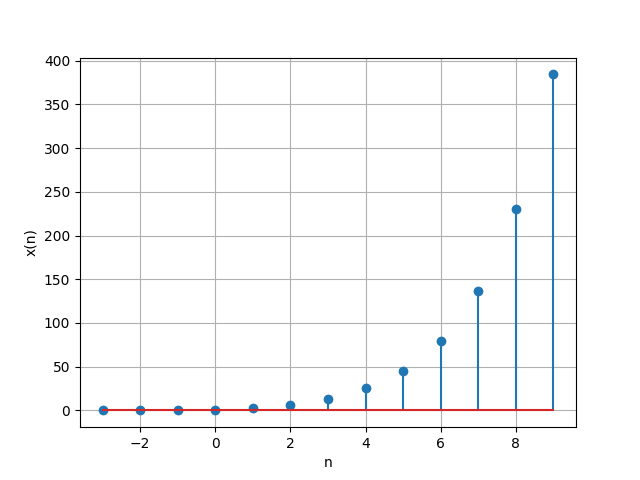
\includegraphics[width = \columnwidth]{2021/EE/31/figs/transform.png}
	\caption{$x(n) vs n $ using $a = 1.5$}
    \label{fig:graph1.41.IN.2022}
\end{figure}


\pagebreak
\end{enumerate}

\section{2021}
\chapter{Systems}
\section{2021}
\begin{enumerate}[label=\thechapter.\arabic*,ref=\thechapter.\theenumi]
\item Two discrete-time linear time-invarient systems with impulse responses $h_1[n]=\delta[n-1]+\delta[n+1]$ and $h_2[n]=\delta[n]+\delta[n-1]$ are connected in cascade, where $\delta[n]$ is the Kronecker delta. The impulse response of the cascaded system is   \\
\begin{enumerate}[label=(\alph*)]
    \item $\delta[n-2]+\delta[n+1]$
    \item $\delta[n-1]\delta[n]+\delta[n+1]\delta[n-1]$
    \item $\delta[n-2]+\delta[n-1]+\delta[n]+\delta[n+1]$
    \item $\delta[n]\delta[n-1]+\delta[n-2]\delta[n+1]$
\end{enumerate} \hfill(GATE 2021 EE)\\
\solution
\iffalse
\let\negmedspace\undefined
\let\negthickspace\undefined
\documentclass[journal,12pt,twocolumn]{IEEEtran}
\usepackage{cite}
\usepackage{amsmath,amssymb,amsfonts,amsthm}
\usepackage{algorithmic}
\usepackage{graphicx}
\usepackage{textcomp}
\usepackage{xcolor}
\usepackage{pgfplots}
\usepackage{txfonts}
\usepackage{listings}
\usepackage{enumitem}
\usepackage{mathtools}
\usepackage{gensymb}
\usepackage{comment}
\usepackage[breaklinks=true]{hyperref}
\usepackage{tkz-euclide} 
\usepackage{listings}
\usepackage{gvv}                                        
\def\inputGnumericTable{}                                 
\usepackage[latin1]{inputenc}                                
\usepackage{color}                                            
\usepackage{array}                                            
\usepackage{longtable}                                       
\usepackage{calc}                                             
\usepackage{multirow}                                         
\usepackage{hhline}                                           
\usepackage{ifthen}                                           
\usepackage{lscape}

\newtheorem{theorem}{Theorem}[section]
\newtheorem{problem}{Problem}
\newtheorem{proposition}{Proposition}[section]
\newtheorem{lemma}{Lemma}[section]
\newtheorem{corollary}[theorem]{Corollary}
\newtheorem{example}{Example}[section]
\newtheorem{definition}[problem]{Definition}
\newcommand{\BEQA}{\begin{eqnarray}}
\newcommand{\EEQA}{\end{eqnarray}}
\newcommand{\define}{\stackrel{\triangle}{=}}
\theoremstyle{remark}
\newtheorem{rem}{Remark}
\begin{document}
\parindent 0px
\bibliographystyle{IEEEtran}
\title{GATE: EE - 7.2021}
\author{EE22BTECH11219 - Rada Sai Sujan$^{}$% <-this % stops a space
}
\maketitle
\newpage
\bigskip
\section*{Question}
Two discrete-time linear time-invarient systems with impulse responses $h_1[n]=\delta[n-1]+\delta[n+1]$ and $h_2[n]=\delta[n]+\delta[n-1]$ are connected in cascade, where $\delta[n]$ is the Kronecker delta. The impulse response of the cascaded system is   \\
\begin{enumerate}[label=(\alph*)]
    \item $\delta[n-2]+\delta[n+1]$
    \item $\delta[n-1]\delta[n]+\delta[n+1]\delta[n-1]$
    \item $\delta[n-2]+\delta[n-1]+\delta[n]+\delta[n+1]$
    \item $\delta[n]\delta[n-1]+\delta[n-2]\delta[n+1]$
\end{enumerate} \hfill(GATE 2021 EE)\\
\solution
\fi

\begin{figure}[ht]
    \centering
    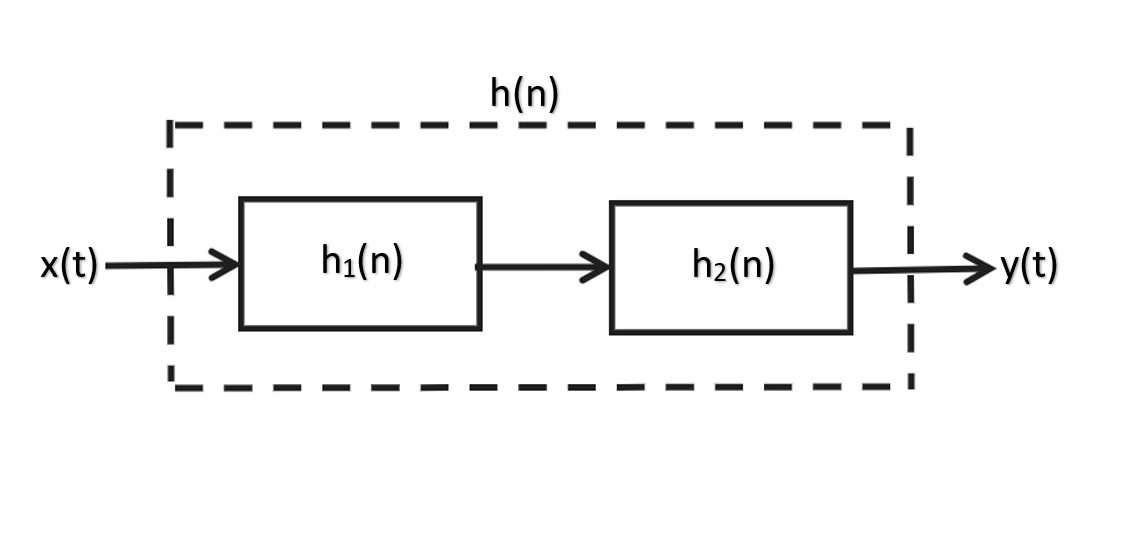
\includegraphics[width=\columnwidth]{2021/EE/7/figs/fig2.png}
    \caption{Block Diagram}
    \label{fig:g2022ee7.2}
\end{figure}  
From the $Z$-transformation pairs,
\begin{align}
    \delta[n] &\overset{\mathcal{Z}}{ \longleftrightarrow} 1  \label{eqn:g22ee7.1}  \\
    x\brak{n-k} &\overset{\mathcal{Z}}{ \longleftrightarrow} z^{-k}X\brak{z} \label{eqn:g22ee7.2}   \\
    x_1\brak{n}\ast x_2\brak{n} &\overset{\mathcal{Z}}{ \longleftrightarrow} X_1\brak{z}X_2\brak{z} \label{eqn:g22ee7.3}
\end{align}
If $h_1\brak{n}$ and $h_2\brak{n}$ are cascade connected then the resultant impulse can be given by:
\begin{align}
    h\brak{n}&=h_1\brak{n}\ast h_2\brak{n}    \\
    \implies H\brak{z}&=H_1\brak{z}H_2\brak{z}    \\
    H\brak{z}&=\brak{z^{-1}+z}\brak{1+z^{-1}}   \\
    &=\brak{z^{-1}+z^{-2}+z+1}, \quad \abs{z}\neq 0
\end{align}
Using the $Z$-transformation pairs to find the the inverse $Z$-transform,
\begin{align}
    h\brak{n}&=\delta[n-2]+\delta[n-1]+\delta[n]+\delta[n+1]
\end{align}
\begin{figure}[ht]
    \centering
    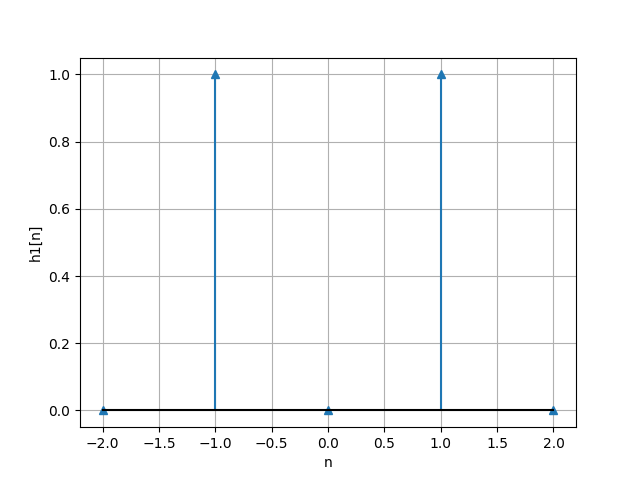
\includegraphics[width=\columnwidth]{2021/EE/7/figs/fig3.png}
    \caption{$h_1\brak{n}$ $vs$ $n$ graph}
    \label{fig:g2022ee7.3}
\end{figure}     
\begin{figure}[ht]
    \centering
    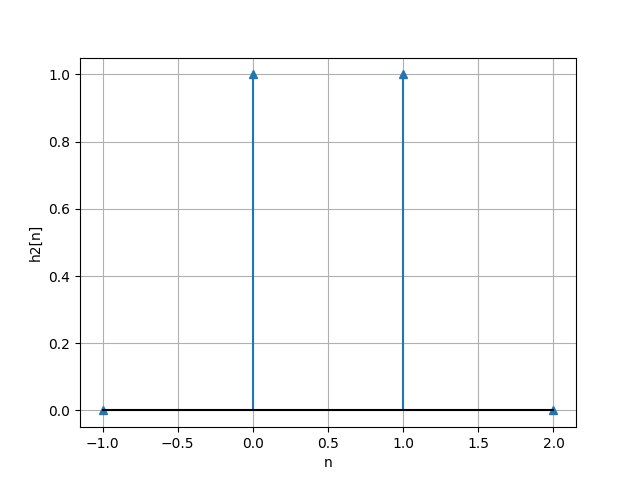
\includegraphics[width=\columnwidth]{2021/EE/7/figs/fig4.png}
    \caption{$h_2\brak{n}$ $vs$ $n$ graph}
    \label{fig:g2022ee7.4}
\end{figure}     
\begin{figure}[ht]
    \centering
    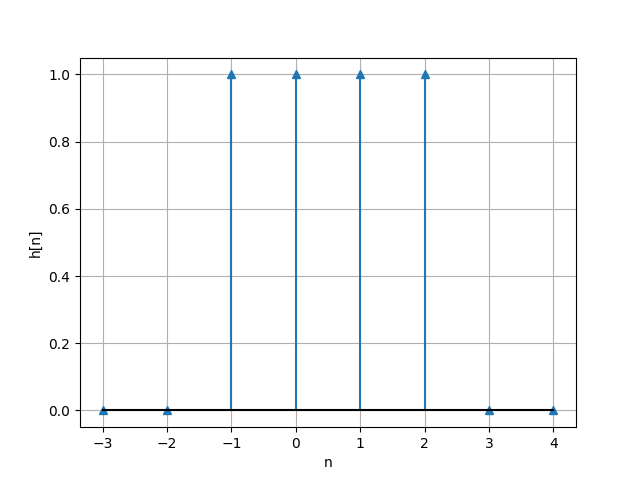
\includegraphics[width=\columnwidth]{2021/EE/7/figs/fig1.png}
    \caption{$h\brak{n}$ $vs$ $n$ graph}
    \label{fig:g2022ee7.1}
\end{figure}

\pagebreak

\item In the given figure, plant $G_p(s)=\frac{2.2}{(1+0.1s)(1+0.4s)(1+1.2s)}$ and compensator $G_c(s)=K\brak{\frac{1+T_1s}{1+T_2s}}$ . The external disturbance input is D(s). It is desired that when the disturbance is a unit step, the steady-state error should not exceed 0.1 unit. The minimum value of K is
\begin{figure}[h!]
    \centering
    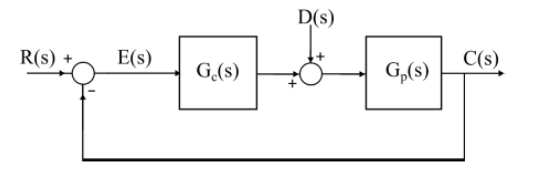
\includegraphics[width=\columnwidth]{2021/EE/47/figs/fig.png}
    \caption{}
    \label{fig:sr47}
\end{figure}
\solution
\iffalse
\documentclass[journal,12pt,twocolumn]{IEEEtran}
\usepackage{cite}
\usepackage{amsmath,amssymb,amsfonts,amsthm}
\usepackage{algorithmic}
\usepackage{graphicx}
\usepackage{textcomp}
\usepackage{xcolor}
\usepackage{txfonts}
\usepackage{listings}
\usepackage{enumitem}
\usepackage{mathtools}
\usepackage{float}
\usepackage{gensymb}
\usepackage{comment}
\usepackage[breaklinks=true]{hyperref}
\usepackage{tkz-euclide} 
\usepackage{listings}
\usepackage{gvv}                                        
\def\inputGnumericTable{}                                 
\usepackage[latin1]{inputenc}                                
\usepackage{color}                                            
\usepackage{array}                                            
\usepackage{longtable}                                       
\usepackage{calc}                                             
\usepackage{multirow}                                         
\usepackage{hhline}                                           
\usepackage{ifthen}                                           
\usepackage{lscape}
\usepackage{amsmath}
\newtheorem{theorem}{Theorem}[section]
\newtheorem{problem}{Problem}
\newtheorem{proposition}{Proposition}[section]
\newtheorem{lemma}{Lemma}[section]
\newtheorem{corollary}[theorem]{Corollary}
\newtheorem{example}{Example}[section]
\newtheorem{definition}[problem]{Definition}
\newcommand{\BEQA}{\begin{eqnarray}}
\newcommand{\EEQA}{\end{eqnarray}}
\newcommand{\define}{\stackrel{\triangle}{=}}
\theoremstyle{remark}
\newtheorem{rem}{Remark}

\usepackage{circuitikz} 

\begin{document}
{\small

\bibliographystyle{IEEEtran}
\vspace{3cm}

\title{GATE 2021 EE 47}
\author{EE23BTECH11045 - Palavelli Srija$^{*}$}

\maketitle

\bigskip

\renewcommand{\thefigure}{\theenumi}
\renewcommand{\thetable}{\theenumi}

\vspace{3cm}
\textbf{Question:} 
In the given figure, plant $G_p(s)=\frac{2.2}{(1+0.1s)(1+0.4s)(1+1.2s)}$ and compensator $G_c(s)=K\brak{\frac{1+T_1s}{1+T_2s}}$ . The external disturbance input is D(s). It is desired that when the disturbance is a unit step, the steady-state error should not exceed 0.1 unit. The minimum value of K is
\begin{figure}[h!]
    \centering
    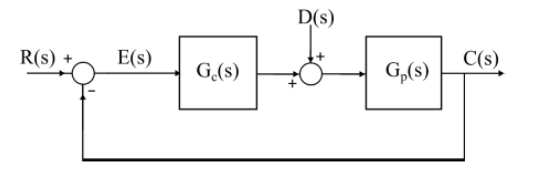
\includegraphics[width=\columnwidth]{2021/EE/47/figs/fig.png}
    \caption{}
    \label{fig:sr40}
\end{figure}
\\
\textbf{Solution:}\\
\fi
\begin{table}[h!]
    \centering
     \begin{tabular}{|c|c|}
        \hline
        \textbf{Symbol}  & \textbf{Value} \\
        \hline
        $G_p(s)$ & $\frac{2.2}{(1+0.1s)(1+0.4s)(1+1.2s)}$\\
         \hline
        $G_c(s)$& $K\brak{\frac{1+T_1s}{1+T_2s}}$  \\
         \hline
        $|e_{ss}|$& $\leq 0.1$\\
         \hline
        $K_{min}$& ??\\
        \hline
    \end{tabular}

    \caption{Input Parameters}
    \label{tab:table_omega}
\end{table}
 
\begin{align}
\text{From \figref{fig:sr40}}\notag\\
E(s) &= R(s)-C(s) \\
\text{Assume R(s)=0}\notag\\
E(s) &= -C(s) \\
C(s) &= \brak{E(s)G_c(s)+D(s)}G_p(s) \\
-E(s) &= \brak{E(s)G_c(s)+D(s)}G_p(s) \\
E(s) &= \frac{-D(s)G_p(s)}{1+G_c(s)G_p(s)} 
\end{align}
Using final value theorem 
\begin{align}
e_{ss} &= \lim_{{t \to \infty}} e(t) = \lim_{{s \to 0}} sE(s)\\
\text{Where}\quad\mathcal{L}\{e(t)\} &= E(s) \notag\\
e_{ss} &= \lim_{{s \to 0}} sE(s) \\
&= \lim_{{s \to 0}} \left(\frac{-sD(s)G_p(s)}{1+G_c(s)G_p(s)} \right) \\
\end{align}
\begin{align}
 D(s)&=\mathcal{L}\{u(t)\}  \notag\\
&=\frac{1}{s}\\
e_{ss} &=\lim_{{s \to 0}} \left(\frac{-s\frac{1}{s}G_p(s)}{1+G_c(s)G_p(s)} \right) \\
&= \lim_{{s \to 0}} \frac{\frac{-2.2}{(1+0.1s)(1+0.4s)(1+1.2s)}}{1+K\left(\frac{1+T_1s}{1+T_2s}\right)\frac{2.2}{(1+0.1s)(1+0.4s)(1+1.2s)}} \\
&= \lim_{{s \to 0}} \frac{-2.2(1+T_2s)}{(1+0.1s)(1+0.4s)(1+1.2s)(1+T_2s)+2.2K(1+T_1s)} \\
|e_{ss}| &= \frac{2.2}{1+2.2K} \\
\text{given}\notag\\ |e_{ss}|&\leq 0.1\\
\frac{2.2}{1+2.2K} &\leq 0.1 \\
K &\geq 9.54 \\
K_{\text{min}} &= 9.54
\end{align}
    %\end{document}

\pagebreak
\end{enumerate}

\section{2021}
\chapter{Sequences}
\section{2021}
\begin{enumerate}[label=\thechapter.\arabic*,ref=\thechapter.\theenumi]
\item 
\solution
\input{}
\pagebreak
\end{enumerate}

\section{2021}
\chapter{Sampling}
\section{2021}
\begin{enumerate}[label=\thechapter.\arabic*,ref=\thechapter.\theenumi]
\item An analog signal is sampled at 100 MHz to generate 1024 samples. Only
these samples are used to evaluate 1024-point FFT. The separation between
adjacent frequency points ($\Delta$F) in FFT is \rule{1cm}{0.5mm} kHz.\\
\hfill (GATE BM 2021)\\
\solution
\iffalse
\documentclass[journal,12pt,twocolumn]{IEEEtran}
\usepackage{amsmath,amssymb,amsfonts,amsthm}
\usepackage{txfonts}
\usepackage{tkz-euclide}
\usepackage{listings}
\usepackage{gvv}
\usepackage[latin1]{inputenc}
\usepackage{adjustbox}
\usepackage{array}
\usepackage{tabularx}
\usepackage{pgf}
\usepackage{lmodern}
\usepackage{circuitikz}
\usepackage{tikz}
\usepackage{graphicx}
\usepackage[english]{babel}

\begin{document}
\bibliographystyle{IEEEtran}

\vspace{3cm}

\title{}
\author{EE23BTECH11047 - Deepakreddy P
}
\maketitle
\newpage
\bigskip

\noindent \textbf{32} \quad An analog signal is sampled at 100 MHz to generate 1024 samples. Only
these samples are used to evaluate 1024-point FFT. The separation between
adjacent frequency points ($\Delta$F) in FFT is \rule{1cm}{0.5mm} kHz.\\
\hfill (GATE BM 2021)\\
\solution
\fi

\begin{center}
    \begin{table}[ht]
        \setlength{\arrayrulewidth}{0.3mm}
\setlength{\tabcolsep}{12pt}
\renewcommand{\arraystretch}{1.3}


\begin{center}
\caption{Input Parameters}
\begin{tabular}{ |p{1.7cm}|p{1.7cm}|p{1.7cm}|  }

\hline
 {Symbol}&{Description} & {value}\\
\hline
$f_s$ & Sampling frequency & 100 MHz\\
\hline
$N$ & No of samples  & 1024\\
\hline

\end{tabular}
\end{center}

    \end{table}
\end{center}

\begin{align}
    \Delta F &= \frac{f_s}{N}\\
    \Delta F &= \frac{100}{1024} MHz\\
    \Delta F &= \frac{10^5}{1024} kHz\\
    \Delta F &= 97.66kHz
\end{align}


\begin{figure}[ht]
   \centering
   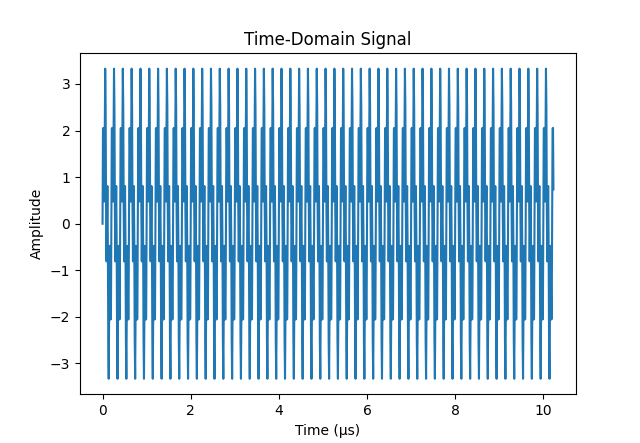
\includegraphics[width=1.1\columnwidth]{2021/BM/32/figs/fig1.png}
   \caption{Time Domain Signal}
\end{figure}

\begin{figure}[ht]
   \centering
   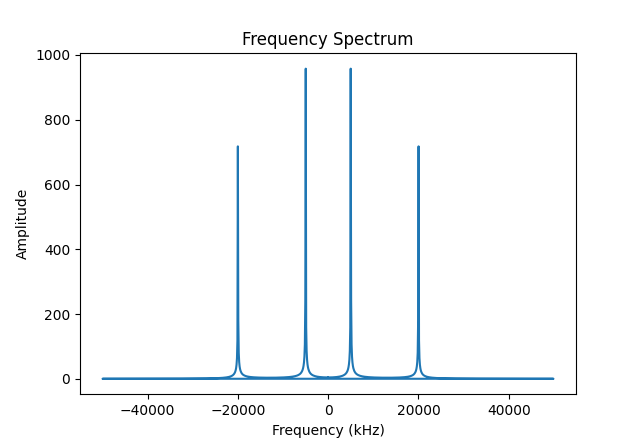
\includegraphics[width=1.1\columnwidth]{2021/BM/32/figs/fig2.png}
   \caption{Frequency Spectrum}
\end{figure}






%\end{document}


\newpage

\item Consider a real-valued base-band signal $x(t)$, band limited to $10kHz$. The Nyquist rate for the signal \\\\
$y(t) = x(t)x(1+\dfrac{t}{2})$ is\\

\begin{enumerate}
\item[(A)] $15kHz$
\item[(B)] $30kHz$
\item[(C)] $60kHz$
\item[(D)] $20kHz$
\end{enumerate}
\hfill{(GATE EC 2021)}\\
\solution
\iffalse
\documentclass[journal,12pt,twocolumn]{IEEEtran}
\usepackage{cite}
\usepackage{amsmath,amssymb,amsfonts,amsthm}
\usepackage{algorithmic}
\usepackage{graphicx}
\usepackage{textcomp}
\usepackage{xcolor}
\usepackage{txfonts}
\usepackage{listings}
\usepackage{enumitem}
\usepackage{mathtools}
\usepackage{gensymb}
\usepackage{comment}
\usepackage[breaklinks=true]{hyperref}
\usepackage{tkz-euclide}
\usepackage{listings}
\usepackage{gvv}
\def\inputGnumericTable{}
\usepackage[latin1]{inputenc}
\usepackage{color}
\usepackage{array}
\usepackage{longtable}
\usepackage{calc}
\usepackage{multirow}
\usepackage{hhline}
\usepackage{ifthen}
\usepackage{lscape}
\usepackage{circuitikz}
\usepackage{geometry}

\newtheorem{theorem}{Theorem}[section]
\newtheorem{problem}{Problem}
\newtheorem{proposition}{Proposition}[section]
\newtheorem{lemma}{Lemma}[section]
\newtheorem{corollary}[theorem]{Corollary}
\newtheorem{example}{Example}[section]
\newtheorem{definition}[problem]{Definition}
\newcommand{\BEQA}{\begin{eqnarray}}
\newcommand{\EEQA}{\end{eqnarray}}
\newcommand{\define}{\stackrel{\triangle}{=}}
\theoremstyle{remark}
\newtheorem{rem}{Remark}

\begin{document}

\bibliographystyle{IEEEtran}
\vspace{3cm}

\title{Gate 2021- EC}
\author{EE23BTECH11058 - Sindam Ananya$^{*}$% <-this % stops a space
}
\maketitle
\newpage
\bigskip

\renewcommand{\thefigure}{\theenumi}
\renewcommand{\thetable}{\theenumi}

\vspace{3cm}
\textbf{Question 4:} 
Consider a real-valued base-band signal $x(t)$, band limited to $10kHz$. The Nyquist rate for the signal \\\\
$y(t) = x(t)x(1+\dfrac{t}{2})$ is\\

\begin{enumerate}
\item[(A)] $15kHz$
\item[(B)] $30kHz$
\item[(C)] $60kHz$
\item[(D)] $20kHz$
\end{enumerate}
\hfill{(GATE EC 2021)}\\
\solution
\fi
\begin{table}[h!]
\centering
\begin{tabular}{|c|c|c|}
\hline
\textbf{Parameter} & \textbf{Value} & \textbf{Description}\\
\hline
$x(t)$ & & base-band signal\\
\hline
$f$ & $10kHz$ & Maximum frequency of $X(f)$\\
\hline
$y(t)$ & $x(t)x(1+\dfrac{t}{2})$ & new signal\\
\hline
$f_{max}$ & & Maximum frequency of $Y(f)$\\
\hline
\end{tabular}

\caption{Input Parameters}
\label{tab:gate2021ec4table}
\end{table}
\begin{align}
x(t) &\xleftrightarrow{\mathcal{F}} X(j\omega)\\
x(at) &\xleftrightarrow{\mathcal{F}} \frac{1}{a}X(j\omega)\\
x(t-t_o) &\xleftrightarrow{\mathcal{F}} e^{-j\omega t_o}X(j\omega)\\
x(1+\frac{t}{2}) &\xleftrightarrow{\mathcal{F}} 2e^{j\omega}X(j2\omega)\\
y(t) &= x(t)x(1+\frac{t}{2})\\
x_1(t)x_2(t) &\xleftrightarrow{\mathcal{F}} X_1(f) * X_2(f)\\
Y(f) &= X(f) * 2e^{j2\pi f}X(2f)
\end{align}
\begin{figure}[h!]
    \centering
    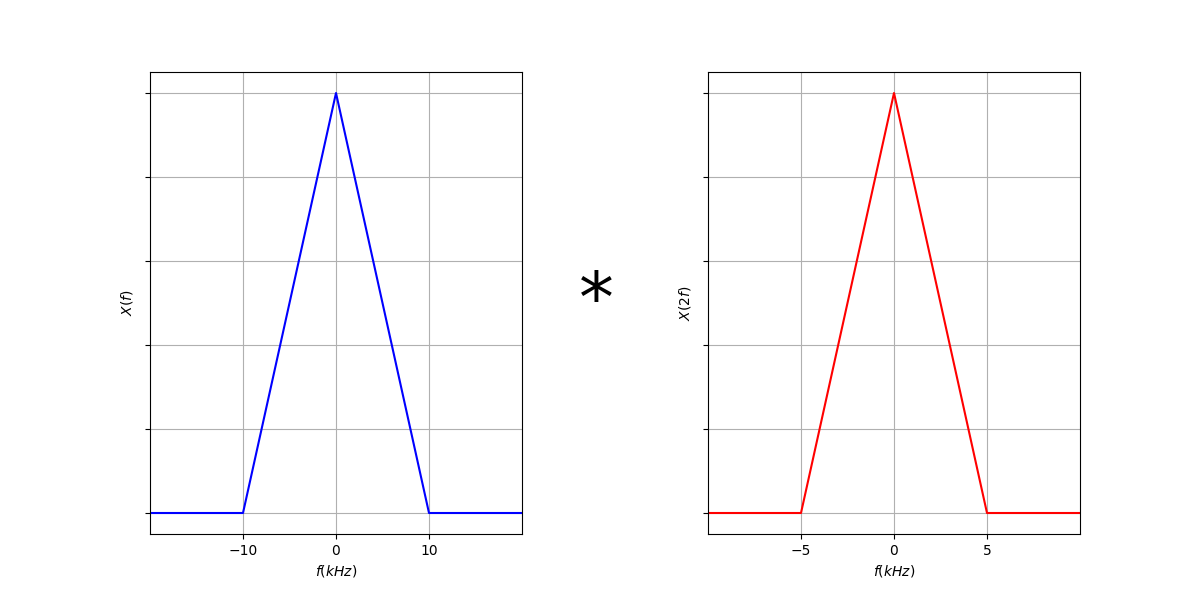
\includegraphics[width=\columnwidth]{2021/EC/4/figs/plot1.png}
    \caption{Plot of $X(f)$ and $X(2f)$}
    \label{fig:gate2021ec4fig1}
\end{figure}
\begin{figure}[h!]
    \centering
    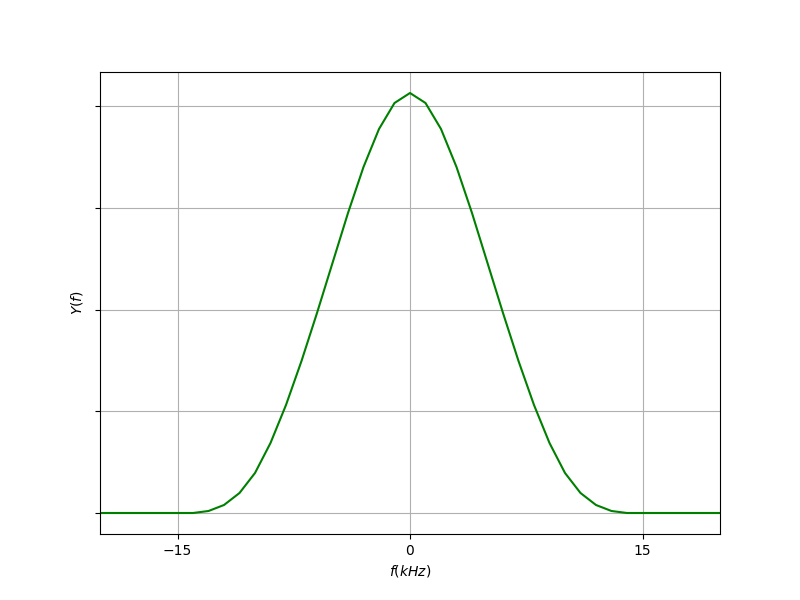
\includegraphics[width=\columnwidth]{2021/EC/4/figs/plot2.png}
    \caption{Plot of $Y(f)$}
    \label{fig:gate2021ec4fig2}
\end{figure}
Nyquist rate is $2f_{max} = 2(15kHz)$ which is $30kHz$
%\end{document}


\newpage

\end{enumerate}

\section{2021}
\chapter{Contour Integration}
\section{2021}
\begin{enumerate}[label=\thechapter.\arabic*,ref=\thechapter.\theenumi]
\item 
\solution
\input{}
\pagebreak
\end{enumerate}

\section{2021}
\chapter{Laplace Transform}
\section{2021}
 \begin{enumerate}[label=\thechapter.\arabic*,ref=\thechapter.\theenumi]
\item For the ordinary differential equation
\begin{align*}
\frac{d^3y}{dt^3} + 6\frac{d^2y}{dt^2} + 11\frac{dy}{dt} + 6y = 1,
\end{align*}
with initial conditions $y(0) = y'(0) = y''(0) = y'''(0) = 0$, the value of 
\begin{align*}
\lim_{{t \to \infty}} y(t) &= ?
\end{align*}
(round off to $3$ decimal places).
\hfill(GATE CH 2021)\\
\solution
\iffalse
\documentclass[journal,12pt,onecolumn]{IEEEtran}
\usepackage{cite}
\usepackage{amsmath,amssymb,amsfonts,amsthm}
\usepackage{algorithmic}
\usepackage{graphicx}
\usepackage{textcomp}
\usepackage{xcolor}
\usepackage{txfonts}
\usepackage{listings}
\usepackage{enumitem}
\usepackage{mathtools}
\usepackage{gensymb}
\usepackage{comment}
\usepackage[breaklinks=true]{hyperref}
\usepackage{tkz-euclide}
\usepackage{braket}
\def\inputGnumericTable{}
\usepackage[latin1]{inputenc}
\usepackage{color}
\usepackage{array}
\usepackage{longtable}
\usepackage{calc}
\usepackage{multirow}
\usepackage{hhline}
\usepackage{ifthen}
\usepackage{lscape}
\usepackage{gvv} 
\usepackage{circuitikz}

\newtheorem{theorem}{Theorem}[section]
\newtheorem{problem}{Problem}
\newtheorem{proposition}{Proposition}[section]
\newtheorem{lemma}{Lemma}[section]
\newtheorem{corollary}[theorem]{Corollary}
\newtheorem{example}{Example}[section]
\newtheorem{definition}[problem]{Definition}
\newcommand{\BEQA}{\begin{eqnarray}}
\newcommand{\EEQA}{\end{eqnarray}}
\newcommand{\define}{\stackrel{\triangle}{=}}
\theoremstyle{remark}
\newtheorem{rem}{Remark}
\renewcommand{\brak}[1]{\left(#1\right)}
\begin{document}

\bibliographystyle{IEEEtran}
\vspace{3cm}

\title{GATE 2021 CH-36}
\author{EE23BTECH11201 - Abburi Tanusha$^{*}$% <-this % stops a space
}
\maketitle

\renewcommand{\thefigure}{\theenumi}
\renewcommand{\thetable}{\theenumi}

\vspace{3cm}

\maketitle
\textbf{Question:} 
For the ordinary differential equation
\begin{align*}
\frac{d^3y}{dt^3} + 6\frac{d^2y}{dt^2} + 11\frac{dy}{dt} + 6y = 1,
\end{align*}
with initial conditions $y(0) = y'(0) = y''(0) = y'''(0) = 0$, the value of 
\begin{align*}
\lim_{{t \to \infty}} y(t) &= ?
\end{align*}
(round off to $3$ decimal places).
\hfill(GATE CH 2021)\\
\textbf{Solution:} 
\fi
\begin{table}[h]
 	\centering
 	\resizebox{6 cm}{!}{
 		
\begin{tabular}{|c|c|l|}
\hline
Parameter  & Value & Description   \\             
\hline
$y(0)$     & $0$   & Initial displacement  \\     
 \hline
$y'(0)$    & $0$   & First derivative at $t=0$  \\
 \hline
$y''(0)$   & $0$   & Second derivative at $t=0$ \\
 \hline
$y'''(0)$  & $0$   & Third derivative at $t=0$  \\
 \hline
\end{tabular}


 	}
 	\vspace{6 pt}
 	\caption{Parameters}
 \end{table}
\begin{align}
\frac{d^3y}{dt^3} + 6\frac{d^2y}{dt^2} + 11\frac{dy}{dt} + 6y &= 1
\end{align}
Applying the Laplace transform to both sides:
\begin{align}
s^3Y(s) + 6s^2Y(s) + 11sY(s) + 6Y(s) &= \frac{1}{s} \\
Y(s)\brak{s^3 + 6s^2 + 11s + 6} &= \frac{1}{s} \\
\implies Y(s) &= \frac{1}{s\brak{s+1}\brak{s+2}\brak{s+3}} ; \quad Re(s) > 0
\end{align}
\begin{align}
Y(s) &= \frac{A}{s} + \frac{B}{s+1} + \frac{C}{s+2} + \frac{D}{s+3} \\
1 &= A\brak{s+1}\brak{s+2}\brak{s+3} + Bs\brak{s+2}\brak{s+3} + Cs\brak{s+1}\brak{s+3} + Ds\brak{s+1}\brak{s+2}  \\
1 &= A\brak{s^3 + 6s^2 + 11s + 6} + Bs\brak{s^2 + 5s + 6}  + Cs\brak{s^2 + 4s + 3} + Ds\brak{s^2 + 3s + 2} \\
\end{align}
Comparing the coefficients on both sides \\
\begin{align}
A + B + C + D = 0 \\
6A + 5B + 4C + 3D = 0 \\
11A + 6B + 3C + 2D = 0 \\
6A = 1 \\
A=1/6 ,B = -11/26 , C= 5/26 , D= 5/78 
\end{align}
Substitute these values 
\begin{align}
Y(s) = \frac{6}{s} - \frac{11}{26\brak{s+1}} + \frac{5}{26\brak{s+2}} + \frac{5}{78\brak{s+3}}
\end{align}
Apply Inverse Laplace Transform 
\begin{align}
y(t) &= 6\mathcal{L}^{-1}\brak{\frac{1}{s}} - 11\mathcal{L}^{-1}\brak{\frac{1}{26\brak{s+1}}} + 5\mathcal{L}^{-1}\brak{\frac{1}{26\brak{s+2}}} + 5\mathcal{L}^{-1}\brak{\frac{1}{78\brak{s+3}}} \\
y(t) &= 6 - \frac{11}{26}e^{-t} + \frac{5}{26}e^{-2t} +\frac{5}{78}e^{-3t}
\end{align}
Consider
\begin{align}
\lim_{t \to \infty} y(t) &= \lim_{t \to \infty} \brak{6 - \frac{11}{26}e^{-t} + \frac{5}{26}e^{-2t} +\frac{5}{78}e^{-3t}} \\
&= 6
\end{align}\
Verifying using Final Value Theorem :\\
\begin{align}
 \lim_{t \to \infty} y(t)   &= \lim_{s \to 0} sY(s)  \\
\lim_{s \to 0} sY(s) &= \lim_{s \to 0} s \brak{ \frac{6}{s} - \frac{11}{26\brak{s+1}} + \frac{5}{26\brak{s+2}} + \frac{5}{78\brak{s+3}}} \\
&= \lim_{s \to 0} \brak{ 6 - \frac{11s}{26\brak{s+1}} + \frac{5s}{26\brak{s+2}} + \frac{5s}{78\brak{s+3}}} \\
&= 6
\end{align}

\begin{figure}[h!]
\centering
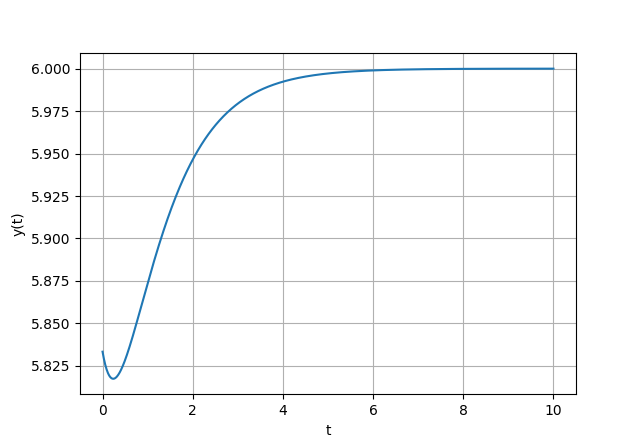
\includegraphics[width=\columnwidth]{2021/CH/36/figs/plot.png}
\caption{Plot $y(t)$ vs $t$ }
\end{figure}
%\end{document}

\pagebreak
\item \textbf{Question:}
Consider the differential equation \\$\frac{d^2y}{dx^2}+8\frac{dy}{dx}+16y=0$ and the boundary conditions $y(0)=1$ and $\frac{dy}{dx}(0)=0$. The solution to equation is:\\
\hfill{(GATE.AE-1.2021)}\\
\solution
 \iffalse
\let\negmedspace\undefined
\let\negthickspace\undefined
\documentclass[journal,12pt,twocolumn]{IEEEtran}
\usepackage{xparse}
\usepackage{cite}
\usepackage{amsmath,amssymb,amsfonts,amsthm}
\usepackage{algorithmic}
\usepackage{graphicx}
\usepackage{textcomp}
\usepackage{xcolor}
\usepackage{txfonts}
\usepackage{listings}
\usepackage{enumitem}
\usepackage{mathtools}
\usepackage{gensymb}
\usepackage{comment}
\usepackage[breaklinks=true]{hyperref}
\usepackage{tkz-euclide}
\usepackage{listings}
\usepackage{gvv}
\def\inputGnumericTable{}
\usepackage[latin1]{inputenc}
\usepackage{color}
\usepackage{array}
\usepackage{longtable}
\usepackage{calc}
\usepackage{multirow}
\usepackage{hhline}
\usepackage{ifthen}
\usepackage{lscape}
\begin{enumerate}[label=\thechapter.\arabic*,ref=\thechapter.\theenumi]
\numberwithin{equation}{enumi}
\numberwithin{figure}{enumi}
\numberwithin{table}{enumi}
\item Laplace Transform of Partial Differentials\\
Let a function $y\brak{x,t}$ be defined for all $t>0$ and assumed to be bounded. Appling Laplace transform in t considering x as a parameter,
\begin{align}
 \mathcal{L}\brak{y\brak{x,t}} &= \int_{0}^{\infty}e^{-st}y\brak{x,t}dt\\
 &= Y\brak{x,s}
\end{align}
Let $\dfrac{\partial y\brak{x,t}}{\partial t}$ be $y_t\brak{x,t}$ and $\dfrac{\partial y\brak{x,t}}{\partial x}$ be $y_x\brak{x,t}$, then
\begin{align}
 \mathcal{L}\brak{y_t\brak{x,t}} &= \int_{0}^{\infty}e^{-st}y_t\brak{x,t}dt\\
 &= \left. e^{-st}y\brak{x,t}\right|_{0}^{\infty} + s\int_{0}^{\infty}e^{-st} y\brak{x,t} dt\\
 &= sY\brak{x,s} - y\brak{x,0} \label{L(y_t(x,t))}\\
 \mathcal{L}\brak{y_x\brak{x,t}} &= \int_{0}^{\infty}e^{-st}y_x\brak{x,t}dt\\
 &= \dfrac{d}{dx}\int_{0}^{\infty}e^{-st}y\brak{x,t}dt \label{L(y_x(x,t))}\\
 &= \dfrac{dY\brak{x,s}}{dx}
\end{align}
\item Laplace transform of f(t):
\begin{align}
        f(t)u(t)\system{L}&\int_{0}^{\infty}f(t)e^{-st}\; dt\\
        &=F(s)\label{lap transform}
\end{align}
\item Laplace transform of powers of $t$\\
        Let $f(t)=t^nu(t)$\\
From \eqref{lap transform},and considering $h=st$
\begin{align}
        F(s)&=\frac{1}{s^{n+1}}\int_{0}^{\infty}h^ne^{-h}\;dh\label{lap 1}\\
        (n-1)!&=\int_0^\infty e^{-t}t^{n-1}\;dt\text{ (Gamma function)}\label{gamma}
\end{align}
From \eqref{lap 1},\eqref{gamma}
\begin{align}
        F(s)&=\frac{n!}{s^{n+1}}\\
         t^nu(t)&\system{L}\frac{n!}{s^{n+1}}\label{lap exp}
\end{align}
\item Frequency shift property:\\
        Let $f(t)=y(t)e^{-at}u(t)$\\
From\eqref{lap transform},
\begin{align}
        F(s)&=\int_0^{\infty}y(t)e^{-(s+a)t}\;dt\\
         y(t)e^{-at}u(t)&\system{L}Y(s+a)\label{lap freq shift}
\end{align}
\item Inverse Laplace for partial fractions\\
From \eqref{lap exp},\eqref{lap freq shift} we get
\begin{align}
    &\frac{b}{(s+a)^n}\xleftrightarrow{\mathcal{L}^{-1}}\frac{b}{(n-1)!}\cdot t^{n-1} e^{-at}\cdot u(t)\label{inv lap (partial fractions)}
\end{align}
\item Laplace transform of derivatives:\\
        Let $f(t)=y'(t)u(t)$\\
From \eqref{lap transform}, integration by parts,recursion
\begin{align}
        F(s)&=\int_{0}^\infty e^{-st}\; dy\\
        &=[y(t)e^{-st}]_0^\infty+s\int_0^\infty y(t)e^{-st}dt\\
        &=-y(0)+sY(s)\label{lap 2}
\end{align}
From\eqref{lap 2},recursion
\begin{align}
        y'(t)u(t)&\system{L}sY(s)-\int y'(t)\;dt\vert_{t=0}\\
        y^{(n)}(t)u(t)&\system{L}s^nY(s)-\sum\limits_{k=0}^{n-1}s^{(n-1-k)}y^{(k)}(0)\label{lap (derivatives)}
\end{align}

\item Laplace transform of integrals:\\
Let the function defined as $y(t) = \int_0^t f(u) du$ for all $t > 0$\\
Laplace transform of y(t) in t 
\begin{align}
    \mathcal{L} \brak{y(t)} &= \int_0^{\infty} e^{-st} y(t) dt\\
    &= \int_0^{\infty} e^{-st} \int_0^t f(u) du dt\\
    &= \int_0^t f(u) du \sbrak{- \frac{e^{-st}}{s}}_0^{\infty} + \int_0^{\infty} \frac{e^{-st}}{s} f(t) dt\\
    &= \frac{F(s)}{s}
\end{align}


\end{enumerate}

\newtheorem{theorem}{Theorem}[section]
\newtheorem{problem}{Problem}
\newtheorem{proposition}{Proposition}[section]
\newtheorem{lemma}{Lemma}[section]
\newtheorem{corollary}[theorem]{Corollary}
\newtheorem{example}{Example}[section]
\newtheorem{definition}[problem]{Definition}
\newcommand{\BEQA}{\begin{eqnarray}}
\newcommand{\EEQA}{\end{eqnarray}}
\newcommand{\define}{\stackrel{\triangle}{=}}
\theoremstyle{remark}
\newtheorem{rem}{Remark}
\begin{document}

\bibliographystyle{IEEEtran}
\vspace{3cm}

\title{GATE-AE.1}
\author{EE23BTECH11046 - Poluri Hemanth$^{*}$}
\maketitle
\textbf{Question:}
Consider the differential equation \\$\frac{d^2y}{dx^2}+8\frac{dy}{dx}+16y=0$ and the boundary conditions $y(0)=1$ and $\frac{dy}{dx}(0)=0$. The solution to equation is:\\
\hfill{(GATE.AE-1.2021)}\\
\textbf{Solution:}\\
\fi
\begin{table}[h!]
    % Change address in github
        %%%%%%%%%%%%%%%%%%%%%%%%%%%%%%%%%%%%%%%%%%%%%%%%%%%%%%%%%%%%%%%%%%%%%%
%%                                                                  %%
%%  This is the header of a LaTeX2e file exported from Gnumeric.    %%
%%                                                                  %%
%%  This file can be compiled as it stands or included in another   %%
%%  LaTeX document. The table is based on the longtable package so  %%
%%  the longtable options (headers, footers...) can be set in the   %%
%%  preamble section below (see PRAMBLE).                           %%
%%                                                                  %%
%%  To include the file in another, the following two lines must be %%
%%  in the including file:                                          %%
%%        \def\inputGnumericTable{}                                 %%
%%  at the beginning of the file and:                               %%
%%        \input{name-of-this-file.tex}                             %%
%%  where the table is to be placed. Note also that the including   %%
%%  file must use the following packages for the table to be        %%
%%  rendered correctly:                                             %%
%%    \usepackage[latin1]{inputenc}                                 %%
%%    \usepackage{color}                                            %%
%%    \usepackage{array}                                            %%
%%    \usepackage{longtable}                                        %%
%%    \usepackage{calc}                                             %%
%%    \usepackage{multirow}                                         %%
%%    \usepackage{hhline}                                           %%
%%    \usepackage{ifthen}                                           %%
%%  optionally (for landscape tables embedded in another document): %%
%%    \usepackage{lscape}                                           %%
%%                                                                  %%
%%%%%%%%%%%%%%%%%%%%%%%%%%%%%%%%%%%%%%%%%%%%%%%%%%%%%%%%%%%%%%%%%%%%%%



%%  This section checks if we are begin input into another file or  %%
%%  the file will be compiled alone. First use a macro taken from   %%
%%  the TeXbook ex 7.7 (suggestion of Han-Wen Nienhuys).            %%
\def\ifundefined#1{\expandafter\ifx\csname#1\endcsname\relax}


%%  Check for the \def token for inputed files. If it is not        %%
%%  defined, the file will be processed as a standalone and the     %%
%%  preamble will be used.                                          %%
\ifundefined{inputGnumericTable}

%%  We must be able to close or not the document at the end.        %%
	\def\gnumericTableEnd{\end{document}}


%%%%%%%%%%%%%%%%%%%%%%%%%%%%%%%%%%%%%%%%%%%%%%%%%%%%%%%%%%%%%%%%%%%%%%
%%                                                                  %%
%%  This is the PREAMBLE. Change these values to get the right      %%
%%  paper size and other niceties.                                  %%
%%                                                                  %%
%%%%%%%%%%%%%%%%%%%%%%%%%%%%%%%%%%%%%%%%%%%%%%%%%%%%%%%%%%%%%%%%%%%%%%

	\documentclass[12pt%
			  %,landscape%
                    ]{report}
       \usepackage[latin1]{inputenc}
       \usepackage{fullpage}
       \usepackage{color}
       \usepackage{array}
       \usepackage{longtable}
       \usepackage{calc}
       \usepackage{multirow}
       \usepackage{hhline}
       \usepackage{ifthen}

	\begin{document}


%%  End of the preamble for the standalone. The next section is for %%
%%  documents which are included into other LaTeX2e files.          %%
\else

%%  We are not a stand alone document. For a regular table, we will %%
%%  have no preamble and only define the closing to mean nothing.   %%
    \def\gnumericTableEnd{}

%%  If we want landscape mode in an embedded document, comment out  %%
%%  the line above and uncomment the two below. The table will      %%
%%  begin on a new page and run in landscape mode.                  %%
%       \def\gnumericTableEnd{\end{landscape}}
%       \begin{landscape}


%%  End f the else clause for this file being \input.              %%
\fi

%%%%%%%%%%%%%%%%%%%%%%%%%%%%%%%%%%%%%%%%%%%%%%%%%%%%%%%%%%%%%%%%%%%%%%
%%                                                                  %%
%%  The rest is the gnumeric table, except for the closing          %%
%%  statement. Changes below will alter the table's appearance.     %%
%%                                                                  %%
%%%%%%%%%%%%%%%%%%%%%%%%%%%%%%%%%%%%%%%%%%%%%%%%%%%%%%%%%%%%%%%%%%%%%%

\providecommand{\gnumericmathit}[1]{#1} 
%%  Uncomment the next line if you would like your numbers to be in %%
%%  italics if they are italizised in the gnumeric table.           %%
%\renewcommand{\gnumericmathit}[1]{\mathit{#1}}
\providecommand{\gnumericPB}[1]%
{\let\gnumericTemp=\\#1\let\\=\gnumericTemp\hspace{0pt}}
 \ifundefined{gnumericTableWidthDefined}
        \newlength{\gnumericTableWidth}
        \newlength{\gnumericTableWidthComplete}
        \newlength{\gnumericMultiRowLength}
        \global\def\gnumericTableWidthDefined{}
 \fi
%% The following setting protects this code from babel shorthands.  %%
 \ifthenelse{\isundefined{\languageshorthands}}{}{\languageshorthands{english}}
%%  The default table format retains the relative column widths of  %%
%%  gnumeric. They can easily be changed to c, r or l. In that case %%
%%  you may want to comment out the next line and uncomment the one %%
%%  thereafter                                                      %%
\providecommand\gnumbox{\makebox[0pt]}
%%\providecommand\gnumbox[1][]{\makebox}

%% to adjust positions in multirow situations                       %%
\setlength{\bigstrutjot}{\jot}
\setlength{\extrarowheight}{\doublerulesep}

%%  The \setlongtables command keeps column widths the same across  %%
%%  pages. Simply comment out next line for varying column widths.  %%
\setlongtables

\setlength\gnumericTableWidth{%
	20pt+%
	40pt+%
	50pt+%	
0pt}
\def\gumericNumCols{3}
\setlength\gnumericTableWidthComplete{\gnumericTableWidth+%
         \tabcolsep*\gumericNumCols*2+\arrayrulewidth*\gumericNumCols}
\ifthenelse{\lengthtest{\gnumericTableWidthComplete > \linewidth}}%
         {\def\gnumericScale{1*\ratio{\linewidth-%
                        \tabcolsep*\gumericNumCols*2-%
                        \arrayrulewidth*\gumericNumCols}%
{\gnumericTableWidth}}}%
{\def\gnumericScale{2}}

%%%%%%%%%%%%%%%%%%%%%%%%%%%%%%%%%%%%%%%%%%%%%%%%%%%%%%%%%%%%%%%%%%%%%%
%%                                                                  %%
%% The following are the widths of the various columns. We are      %%
%% defining them here because then they are easier to change.       %%
%% Depending on the cell formats we may use them more than once.    %%
%%                                                                  %%
%%%%%%%%%%%%%%%%%%%%%%%%%%%%%%%%%%%%%%%%%%%%%%%%%%%%%%%%%%%%%%%%%%%%%%

\ifthenelse{\isundefined{\gnumericColA}}{\newlength{\gnumericColA}}{}\settowidth{\gnumericColA}{\begin{tabular}{@{}p{20pt*\gnumericScale}@{}}x\end{tabular}}
\ifthenelse{\isundefined{\gnumericColB}}{\newlength{\gnumericColB}}{}\settowidth{\gnumericColB}{\begin{tabular}{@{}p{40pt*\gnumericScale}@{}}x\end{tabular}}
\ifthenelse{\isundefined{\gnumericColC}}{\newlength{\gnumericColC}}{}\settowidth{\gnumericColC}{\begin{tabular}{@{}p{50pt*\gnumericScale}@{}}x\end{tabular}}

\begin{tabular}[c]{%
	b{\gnumericColA}%
	b{\gnumericColB}%
	b{\gnumericColC}%
	}

%%%%%%%%%%%%%%%%%%%%%%%%%%%%%%%%%%%%%%%%%%%%%%%%%%%%%%%%%%%%%%%%%%%%%%
%%  The longtable options. (Caption, headers... see Goosens, p.124) %%
%	\caption{The Table Caption.}             \\	%
% \hline	% Across the top of the table.
%%  The rest of these options are table rows which are placed on    %%
%%  the first, last or every page. Use \multicolumn if you want.    %%

%%  Header for the first page.                                      %%
%	\multicolumn{3}{c}{The First Header} \\ \hline 
%	\multicolumn{1}{c}{colTag}	%Column 1
%	&\multicolumn{1}{c}{colTag}	%Column 2
%	&\multicolumn{1}{c}{colTag}	\\ \hline %Last column
%	\endfirsthead

%%  The running header definition.                                  %%
%	\hline
%	\multicolumn{3}{l}{\ldots\small\slshape continued} \\ \hline
%	\multicolumn{1}{c}{colTag}	%Column 1
%	&\multicolumn{1}{c}{colTag}	%Column 2
%	&\multicolumn{1}{c}{colTag}	\\ \hline %Last column
%	\endhead

%%  The running footer definition.                                  %%
%	\hline
%	\multicolumn{3}{r}{\small\slshape continued\ldots} \\
%	\endfoot

%%  The ending footer definition.                                   %%
%	\multicolumn{3}{c}{That's all folks} \\ \hline 
%	\endlastfoot
%%%%%%%%%%%%%%%%%%%%%%%%%%%%%%%%%%%%%%%%%%%%%%%%%%%%%%%%%%%%%%%%%%%%%%
\hhline{|-|-|-}
	\multicolumn{1}{|p{\gnumericColA}|}%
	{\gnumericPB{\centering}\gnumbox{\textbf{Symbol}}}
	&\multicolumn{1}{p{\gnumericColB}|}%
	{\gnumericPB{\centering}\gnumbox{\textbf{Values}}}
	&\multicolumn{1}{p{\gnumericColC}|}%
	{\gnumericPB{\centering}\gnumbox{\textbf{Description}}}

\\
\hhline{|---|}
	\multicolumn{1}{|p{\gnumericColA}|}%
	{\gnumericPB{\centering}\gnumbox{$Y(s)$}}
	&\multicolumn{1}{p{\gnumericColB}|}%
	{\gnumericPB{\centering}\gnumbox{-}}
	&\multicolumn{1}{p{\gnumericColC}|}%
	{\gnumericPB{\centering}\gnumbox{$y$ in s domain}}

\\
\hhline{|---|}
        \multicolumn{1}{|p{\gnumericColA}|}%
	{\gnumericPB{\centering}\gnumbox{$y(x)$}}             
        &\multicolumn{1}{p{\gnumericColB}|}%
	{\gnumericPB{\centering}\gnumbox{-}}  
        &\multicolumn{1}{p{\gnumericColC}|}%
	{\gnumericPB{\centering}\gnumbox{$y$ in x domain}}

\\
\hhline{|---|}
        \multicolumn{1}{|p{\gnumericColA}|}%
        {\gnumericPB{\centering}\gnumbox{$y(0)$}}             
        &\multicolumn{1}{p{\gnumericColB}|}%
        {\gnumericPB{\centering}\gnumbox{1}}  
        &\multicolumn{1}{p{\gnumericColC}|}%
        {\gnumericPB{\centering}\gnumbox{$y$ at $x=0$}}
\\
\hhline{|---|}
        \multicolumn{1}{|p{\gnumericColA}|}%
        {\gnumericPB{\centering}\gnumbox{$y'(0)$}}             
        &\multicolumn{1}{p{\gnumericColB}|}%
        {\gnumericPB{\centering}\gnumbox{0}}  
        &\multicolumn{1}{p{\gnumericColC}|}%
	{\gnumericPB{\centering}\gnumbox{$y'(x)$ at $x=0$}}

\\
\hhline{|---|}
        \multicolumn{1}{|p{\gnumericColA}|}%
	{\gnumericPB{\centering}\gnumbox{$u(x)$}}             
        &\multicolumn{1}{p{\gnumericColB}|}%
	{\gnumericPB{\centering}\gnumbox{$=\begin{cases}
        1 & \text{if } x > 0\\
        0 &  o.w
    \end{cases}$}}  
        &\multicolumn{1}{p{\gnumericColC}|}%
        {\gnumericPB{\centering}\gnumbox{unit step function}}
\\
\hhline{|-|-|-|}
\end{tabular}

\ifthenelse{\isundefined{\languageshorthands}}{}{\languageshorthands{\languagename}}
\gnumericTableEnd

        \caption{Parameters}
        \label{tab:AE.1.2021}
\end{table}\\
From \ref{lap (derivatives)}
\begin{align}
	\frac{d^2y}{dx^2}+8\frac{dy}{dx}+16y&\Large\xleftrightarrow{\mathcal{L}}s^2Y(s)-sy(0)-y'(0)+8sY(s)-8y(0)+16Y(s)
\end{align}
\begin{align}
	Y(s)(s^2+8s+16)&=s+8
\end{align}
\begin{align}
	\Rightarrow Y(s)&=\frac{s+8}{s^2+8s+16}\\
	&=\frac{1}{s+4}+\frac{4}{(s+4)^2}\label{1ae.1}
\end{align}
For inversion of $Y(s)$ in partial fractions-
\\ From \ref{inv lap (partial fractions)}
\begin{align}
	&\frac{b}{(s+a)^n}\Large\xleftrightarrow{\mathcal{L}^{-1}}\frac{b}{(n-1)!}\cdot x^{n-1} e^{-ax}\cdot u(x)\label{invae.1}
\end{align}
\\
Applying Laplace inverse-\\
\\From \eqref{1ae.1},\eqref{invae.1}
\begin{align}
	y(x)&=\frac{1}{0!} e^{-4x}\cdot u(x)+\frac{4}{1!}x\cdot e^{-4x}\cdot u(x)\\
	&=(1+4x)e^{-4x}u(x)
\end{align}
\newpage
\begin{figure}[h!]
    \centering
    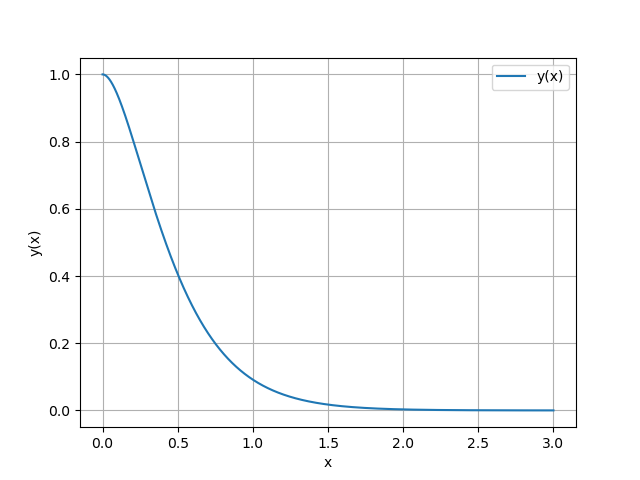
\includegraphics[width=1\linewidth]{2021/AE/1/figures/figure.png}
        \caption{Plot of y(x)}
    \label{fig:enter-label}
\end{figure}


%\end{document}






\pagebreak
\item\textbf{Question:}
The solution of second-order differential equation \\ $\frac{d^2y}{dx^2}+2\frac{dy}{dx}+y=0$ with boundary conditions $y(0)=1$ and $y(1)=3$.\\
\hfill{(GATE  2021 CE.26)}\\
\solution
\iffalse
\let\negmedspace\undefined
\let\negthickspace\undefined
\documentclass[journal,12pt,twocolumn]{IEEEtran}
\usepackage{xparse}
\usepackage{cite}
\usepackage{amsmath,amssymb,amsfonts,amsthm}
\usepackage{algorithmic}
\usepackage{graphicx}
\usepackage{textcomp}
\usepackage{xcolor}
\usepackage{txfonts}
\usepackage{listings}
\usepackage{enumitem}
\usepackage{mathtools}
\usepackage{gensymb}
\usepackage{comment}
\usepackage[breaklinks=true]{hyperref}
\usepackage{tkz-euclide}
\usepackage{listings}
\usepackage{gvv}
\def\inputGnumericTable{}
\usepackage[latin1]{inputenc}
\usepackage{color}
\usepackage{array}
\usepackage{longtable}
\usepackage{calc}
\usepackage{multirow}
\usepackage{hhline}
\usepackage{ifthen}
\usepackage{lscape}
\begin{enumerate}[label=\thechapter.\arabic*,ref=\thechapter.\theenumi]
\numberwithin{equation}{enumi}
\numberwithin{figure}{enumi}
\numberwithin{table}{enumi}
\item Laplace Transform of Partial Differentials\\
Let a function $y\brak{x,t}$ be defined for all $t>0$ and assumed to be bounded. Appling Laplace transform in t considering x as a parameter,
\begin{align}
 \mathcal{L}\brak{y\brak{x,t}} &= \int_{0}^{\infty}e^{-st}y\brak{x,t}dt\\
 &= Y\brak{x,s}
\end{align}
Let $\dfrac{\partial y\brak{x,t}}{\partial t}$ be $y_t\brak{x,t}$ and $\dfrac{\partial y\brak{x,t}}{\partial x}$ be $y_x\brak{x,t}$, then
\begin{align}
 \mathcal{L}\brak{y_t\brak{x,t}} &= \int_{0}^{\infty}e^{-st}y_t\brak{x,t}dt\\
 &= \left. e^{-st}y\brak{x,t}\right|_{0}^{\infty} + s\int_{0}^{\infty}e^{-st} y\brak{x,t} dt\\
 &= sY\brak{x,s} - y\brak{x,0} \label{L(y_t(x,t))}\\
 \mathcal{L}\brak{y_x\brak{x,t}} &= \int_{0}^{\infty}e^{-st}y_x\brak{x,t}dt\\
 &= \dfrac{d}{dx}\int_{0}^{\infty}e^{-st}y\brak{x,t}dt \label{L(y_x(x,t))}\\
 &= \dfrac{dY\brak{x,s}}{dx}
\end{align}
\item Laplace transform of f(t):
\begin{align}
        f(t)u(t)\system{L}&\int_{0}^{\infty}f(t)e^{-st}\; dt\\
        &=F(s)\label{lap transform}
\end{align}
\item Laplace transform of powers of $t$\\
        Let $f(t)=t^nu(t)$\\
From \eqref{lap transform},and considering $h=st$
\begin{align}
        F(s)&=\frac{1}{s^{n+1}}\int_{0}^{\infty}h^ne^{-h}\;dh\label{lap 1}\\
        (n-1)!&=\int_0^\infty e^{-t}t^{n-1}\;dt\text{ (Gamma function)}\label{gamma}
\end{align}
From \eqref{lap 1},\eqref{gamma}
\begin{align}
        F(s)&=\frac{n!}{s^{n+1}}\\
         t^nu(t)&\system{L}\frac{n!}{s^{n+1}}\label{lap exp}
\end{align}
\item Frequency shift property:\\
        Let $f(t)=y(t)e^{-at}u(t)$\\
From\eqref{lap transform},
\begin{align}
        F(s)&=\int_0^{\infty}y(t)e^{-(s+a)t}\;dt\\
         y(t)e^{-at}u(t)&\system{L}Y(s+a)\label{lap freq shift}
\end{align}
\item Inverse Laplace for partial fractions\\
From \eqref{lap exp},\eqref{lap freq shift} we get
\begin{align}
    &\frac{b}{(s+a)^n}\xleftrightarrow{\mathcal{L}^{-1}}\frac{b}{(n-1)!}\cdot t^{n-1} e^{-at}\cdot u(t)\label{inv lap (partial fractions)}
\end{align}
\item Laplace transform of derivatives:\\
        Let $f(t)=y'(t)u(t)$\\
From \eqref{lap transform}, integration by parts,recursion
\begin{align}
        F(s)&=\int_{0}^\infty e^{-st}\; dy\\
        &=[y(t)e^{-st}]_0^\infty+s\int_0^\infty y(t)e^{-st}dt\\
        &=-y(0)+sY(s)\label{lap 2}
\end{align}
From\eqref{lap 2},recursion
\begin{align}
        y'(t)u(t)&\system{L}sY(s)-\int y'(t)\;dt\vert_{t=0}\\
        y^{(n)}(t)u(t)&\system{L}s^nY(s)-\sum\limits_{k=0}^{n-1}s^{(n-1-k)}y^{(k)}(0)\label{lap (derivatives)}
\end{align}

\item Laplace transform of integrals:\\
Let the function defined as $y(t) = \int_0^t f(u) du$ for all $t > 0$\\
Laplace transform of y(t) in t 
\begin{align}
    \mathcal{L} \brak{y(t)} &= \int_0^{\infty} e^{-st} y(t) dt\\
    &= \int_0^{\infty} e^{-st} \int_0^t f(u) du dt\\
    &= \int_0^t f(u) du \sbrak{- \frac{e^{-st}}{s}}_0^{\infty} + \int_0^{\infty} \frac{e^{-st}}{s} f(t) dt\\
    &= \frac{F(s)}{s}
\end{align}


\end{enumerate}

\newtheorem{theorem}{Theorem}[section]
\newtheorem{problem}{Problem}
\newtheorem{proposition}{Proposition}[section]
\newtheorem{lemma}{Lemma}[section]
\newtheorem{corollary}[theorem]{Corollary}
\newtheorem{example}{Example}[section]
\newtheorem{definition}[problem]{Definition}
\newcommand{\BEQA}{\begin{eqnarray}}
\newcommand{\EEQA}{\end{eqnarray}}
\newcommand{\define}{\stackrel{\triangle}{=}}
\theoremstyle{remark}
\newtheorem{rem}{Remark}
\begin{document}

\bibliographystyle{IEEEtran}
\vspace{3cm}

\title{GATE-CE.26}
\author{EE23BTECH11046 - Poluri Hemanth$^{*}$}
\maketitle
\textbf{Question:}
The solution of second-order differential equation \\ $\frac{d^2y}{dx^2}+2\frac{dy}{dx}+y=0$ with boundary conditions $y(0)=1$ and $y(1)=3$.\\
\hfill{(GATE  2021 CE.26)}\\
\textbf{Solution:}
\fi
\begin{table}[h!]
    % Change address in github
        %%%%%%%%%%%%%%%%%%%%%%%%%%%%%%%%%%%%%%%%%%%%%%%%%%%%%%%%%%%%%%%%%%%%%%
%%                                                                  %%
%%  This is the header of a LaTeX2e file exported from Gnumeric.    %%
%%                                                                  %%
%%  This file can be compiled as it stands or included in another   %%
%%  LaTeX document. The table is based on the longtable package so  %%
%%  the longtable options (headers, footers...) can be set in the   %%
%%  preamble section below (see PRAMBLE).                           %%
%%                                                                  %%
%%  To include the file in another, the following two lines must be %%
%%  in the including file:                                          %%
%%        \def\inputGnumericTable{}                                 %%
%%  at the beginning of the file and:                               %%
%%        \input{name-of-this-file.tex}                             %%
%%  where the table is to be placed. Note also that the including   %%
%%  file must use the following packages for the table to be        %%
%%  rendered correctly:                                             %%
%%    \usepackage[latin1]{inputenc}                                 %%
%%    \usepackage{color}                                            %%
%%    \usepackage{array}                                            %%
%%    \usepackage{longtable}                                        %%
%%    \usepackage{calc}                                             %%
%%    \usepackage{multirow}                                         %%
%%    \usepackage{hhline}                                           %%
%%    \usepackage{ifthen}                                           %%
%%  optionally (for landscape tables embedded in another document): %%
%%    \usepackage{lscape}                                           %%
%%                                                                  %%
%%%%%%%%%%%%%%%%%%%%%%%%%%%%%%%%%%%%%%%%%%%%%%%%%%%%%%%%%%%%%%%%%%%%%%



%%  This section checks if we are begin input into another file or  %%
%%  the file will be compiled alone. First use a macro taken from   %%
%%  the TeXbook ex 7.7 (suggestion of Han-Wen Nienhuys).            %%
\def\ifundefined#1{\expandafter\ifx\csname#1\endcsname\relax}


%%  Check for the \def token for inputed files. If it is not        %%
%%  defined, the file will be processed as a standalone and the     %%
%%  preamble will be used.                                          %%
\ifundefined{inputGnumericTable}

%%  We must be able to close or not the document at the end.        %%
	\def\gnumericTableEnd{\end{document}}


%%%%%%%%%%%%%%%%%%%%%%%%%%%%%%%%%%%%%%%%%%%%%%%%%%%%%%%%%%%%%%%%%%%%%%
%%                                                                  %%
%%  This is the PREAMBLE. Change these values to get the right      %%
%%  paper size and other niceties.                                  %%
%%                                                                  %%
%%%%%%%%%%%%%%%%%%%%%%%%%%%%%%%%%%%%%%%%%%%%%%%%%%%%%%%%%%%%%%%%%%%%%%

	\documentclass[12pt%
			  %,landscape%
                    ]{report}
       \usepackage[latin1]{inputenc}
       \usepackage{fullpage}
       \usepackage{color}
       \usepackage{array}
       \usepackage{longtable}
       \usepackage{calc}
       \usepackage{multirow}
       \usepackage{hhline}
       \usepackage{ifthen}

	\begin{document}


%%  End of the preamble for the standalone. The next section is for %%
%%  documents which are included into other LaTeX2e files.          %%
\else

%%  We are not a stand alone document. For a regular table, we will %%
%%  have no preamble and only define the closing to mean nothing.   %%
    \def\gnumericTableEnd{}

%%  If we want landscape mode in an embedded document, comment out  %%
%%  the line above and uncomment the two below. The table will      %%
%%  begin on a new page and run in landscape mode.                  %%
%       \def\gnumericTableEnd{\end{landscape}}
%       \begin{landscape}


%%  End f the else clause for this file being \input.              %%
\fi

%%%%%%%%%%%%%%%%%%%%%%%%%%%%%%%%%%%%%%%%%%%%%%%%%%%%%%%%%%%%%%%%%%%%%%
%%                                                                  %%
%%  The rest is the gnumeric table, except for the closing          %%
%%  statement. Changes below will alter the table's appearance.     %%
%%                                                                  %%
%%%%%%%%%%%%%%%%%%%%%%%%%%%%%%%%%%%%%%%%%%%%%%%%%%%%%%%%%%%%%%%%%%%%%%

\providecommand{\gnumericmathit}[1]{#1} 
%%  Uncomment the next line if you would like your numbers to be in %%
%%  italics if they are italizised in the gnumeric table.           %%
%\renewcommand{\gnumericmathit}[1]{\mathit{#1}}
\providecommand{\gnumericPB}[1]%
{\let\gnumericTemp=\\#1\let\\=\gnumericTemp\hspace{0pt}}
 \ifundefined{gnumericTableWidthDefined}
        \newlength{\gnumericTableWidth}
        \newlength{\gnumericTableWidthComplete}
        \newlength{\gnumericMultiRowLength}
        \global\def\gnumericTableWidthDefined{}
 \fi
%% The following setting protects this code from babel shorthands.  %%
 \ifthenelse{\isundefined{\languageshorthands}}{}{\languageshorthands{english}}
%%  The default table format retains the relative column widths of  %%
%%  gnumeric. They can easily be changed to c, r or l. In that case %%
%%  you may want to comment out the next line and uncomment the one %%
%%  thereafter                                                      %%
\providecommand\gnumbox{\makebox[0pt]}
%%\providecommand\gnumbox[1][]{\makebox}

%% to adjust positions in multirow situations                       %%
\setlength{\bigstrutjot}{\jot}
\setlength{\extrarowheight}{\doublerulesep}

%%  The \setlongtables command keeps column widths the same across  %%
%%  pages. Simply comment out next line for varying column widths.  %%
\setlongtables

\setlength\gnumericTableWidth{%
	20pt+%
	40pt+%
	50pt+%	
0pt}
\def\gumericNumCols{3}
\setlength\gnumericTableWidthComplete{\gnumericTableWidth+%
         \tabcolsep*\gumericNumCols*2+\arrayrulewidth*\gumericNumCols}
\ifthenelse{\lengthtest{\gnumericTableWidthComplete > \linewidth}}%
         {\def\gnumericScale{1*\ratio{\linewidth-%
                        \tabcolsep*\gumericNumCols*2-%
                        \arrayrulewidth*\gumericNumCols}%
{\gnumericTableWidth}}}%
{\def\gnumericScale{2}}

%%%%%%%%%%%%%%%%%%%%%%%%%%%%%%%%%%%%%%%%%%%%%%%%%%%%%%%%%%%%%%%%%%%%%%
%%                                                                  %%
%% The following are the widths of the various columns. We are      %%
%% defining them here because then they are easier to change.       %%
%% Depending on the cell formats we may use them more than once.    %%
%%                                                                  %%
%%%%%%%%%%%%%%%%%%%%%%%%%%%%%%%%%%%%%%%%%%%%%%%%%%%%%%%%%%%%%%%%%%%%%%

\ifthenelse{\isundefined{\gnumericColA}}{\newlength{\gnumericColA}}{}\settowidth{\gnumericColA}{\begin{tabular}{@{}p{20pt*\gnumericScale}@{}}x\end{tabular}}
\ifthenelse{\isundefined{\gnumericColB}}{\newlength{\gnumericColB}}{}\settowidth{\gnumericColB}{\begin{tabular}{@{}p{40pt*\gnumericScale}@{}}x\end{tabular}}
\ifthenelse{\isundefined{\gnumericColC}}{\newlength{\gnumericColC}}{}\settowidth{\gnumericColC}{\begin{tabular}{@{}p{50pt*\gnumericScale}@{}}x\end{tabular}}

\begin{tabular}[c]{%
	b{\gnumericColA}%
	b{\gnumericColB}%
	b{\gnumericColC}%
	}

%%%%%%%%%%%%%%%%%%%%%%%%%%%%%%%%%%%%%%%%%%%%%%%%%%%%%%%%%%%%%%%%%%%%%%
%%  The longtable options. (Caption, headers... see Goosens, p.124) %%
%	\caption{The Table Caption.}             \\	%
% \hline	% Across the top of the table.
%%  The rest of these options are table rows which are placed on    %%
%%  the first, last or every page. Use \multicolumn if you want.    %%

%%  Header for the first page.                                      %%
%	\multicolumn{3}{c}{The First Header} \\ \hline 
%	\multicolumn{1}{c}{colTag}	%Column 1
%	&\multicolumn{1}{c}{colTag}	%Column 2
%	&\multicolumn{1}{c}{colTag}	\\ \hline %Last column
%	\endfirsthead

%%  The running header definition.                                  %%
%	\hline
%	\multicolumn{3}{l}{\ldots\small\slshape continued} \\ \hline
%	\multicolumn{1}{c}{colTag}	%Column 1
%	&\multicolumn{1}{c}{colTag}	%Column 2
%	&\multicolumn{1}{c}{colTag}	\\ \hline %Last column
%	\endhead

%%  The running footer definition.                                  %%
%	\hline
%	\multicolumn{3}{r}{\small\slshape continued\ldots} \\
%	\endfoot

%%  The ending footer definition.                                   %%
%	\multicolumn{3}{c}{That's all folks} \\ \hline 
%	\endlastfoot
%%%%%%%%%%%%%%%%%%%%%%%%%%%%%%%%%%%%%%%%%%%%%%%%%%%%%%%%%%%%%%%%%%%%%%
\hhline{|-|-|-}
	\multicolumn{1}{|p{\gnumericColA}|}%
	{\gnumericPB{\centering}\gnumbox{\textbf{Symbol}}}
	&\multicolumn{1}{p{\gnumericColB}|}%
	{\gnumericPB{\centering}\gnumbox{\textbf{Values}}}
	&\multicolumn{1}{p{\gnumericColC}|}%
	{\gnumericPB{\centering}\gnumbox{\textbf{Description}}}

\\
\hhline{|---|}
	\multicolumn{1}{|p{\gnumericColA}|}%
	{\gnumericPB{\centering}\gnumbox{$Y(s)$}}
	&\multicolumn{1}{p{\gnumericColB}|}%
	{\gnumericPB{\centering}\gnumbox{-}}
	&\multicolumn{1}{p{\gnumericColC}|}%
	{\gnumericPB{\centering}\gnumbox{$y$ in s domain}}

\\
\hhline{|---|}
        \multicolumn{1}{|p{\gnumericColA}|}%
	{\gnumericPB{\centering}\gnumbox{$y(x)$}}             
        &\multicolumn{1}{p{\gnumericColB}|}%
	{\gnumericPB{\centering}\gnumbox{-}}  
        &\multicolumn{1}{p{\gnumericColC}|}%
	{\gnumericPB{\centering}\gnumbox{$y$ in x domain}}

\\
\hhline{|---|}
        \multicolumn{1}{|p{\gnumericColA}|}%
        {\gnumericPB{\centering}\gnumbox{$y(0)$}}             
        &\multicolumn{1}{p{\gnumericColB}|}%
        {\gnumericPB{\centering}\gnumbox{1}}  
        &\multicolumn{1}{p{\gnumericColC}|}%
        {\gnumericPB{\centering}\gnumbox{$y$ at $x=0$}}
\\
\hhline{|---|}
        \multicolumn{1}{|p{\gnumericColA}|}%
        {\gnumericPB{\centering}\gnumbox{$y(1)$}}             
        &\multicolumn{1}{p{\gnumericColB}|}%
        {\gnumericPB{\centering}\gnumbox{3}}  
        &\multicolumn{1}{p{\gnumericColC}|}%
	{\gnumericPB{\centering}\gnumbox{$y(x)$ at $x=1$}}

\\
\hhline{|---|}
        \multicolumn{1}{|p{\gnumericColA}|}%
	{\gnumericPB{\centering}\gnumbox{$u(x)$}}             
        &\multicolumn{1}{p{\gnumericColB}|}%
	{\gnumericPB{\centering}\gnumbox{$=\begin{cases}
        1 & \text{if } x > 0\\
        0 &  o.w
    \end{cases}$}}  
        &\multicolumn{1}{p{\gnumericColC}|}%
        {\gnumericPB{\centering}\gnumbox{unit step function}}
\\
\hhline{|-|-|-|}
\end{tabular}

\ifthenelse{\isundefined{\languageshorthands}}{}{\languageshorthands{\languagename}}
\gnumericTableEnd

        \caption{Parameters}
        \label{tab:es.47}
\end{table}\\
Applying Laplace transform
\\From \ref{lap (derivatives)}
\begin{align}
	\frac{d^2y}{dx^2}+2\frac{dy}{dx}+y&\Large\xleftrightarrow{\mathcal{L}}s^2Y(s)-sy(0)-y'(0)+2sY(s)-2y(0)+Y(s)
\end{align}
\begin{align}
	Y(s)(s^2+2s+1)&=s-2-y'(0)
\end{align}
\begin{align}
	\Rightarrow Y(s)&=\frac{s-2-y'(0)}{s^2+2s+1}\\
	&=\frac{1}{s+1}-\frac{2+y'(0)}{(s+1)^2}\label{1ce.1}
\end{align}
For inversion of $Y(s)$ in partial fractions-
\\From \ref{inv lap (partial fractions)}
\begin{align}
	&\frac{b}{(s+a)^n}\system{L}\frac{b}{(n-1)!}\cdot x^{n-1} e^{-ax}\cdot u(x)\label{invce.26}
\end{align}
Applying Laplace inverse-\\
\\From \eqref{1ce.1},\eqref{invce.26}
\begin{align}
	y(x)&=\frac{1}{0!} e^{-x}\cdot u(x)-\frac{3+y'(0)}{1!}x\cdot e^{-x}\cdot u(x)\\
	&=(1-(3+y'(0))x)e^{-x}u(x)\label{yce.26}
\end{align}
From \eqref{yce.26},
\begin{align}
	y(1)&=(1-3-y'(0))e^{-1}\\
	3&=(1-3-y'(0))e^{-1}\\
	\Rightarrow y'(0)&=-(2+3e)\label{y'0ce.26}
\end{align}
From\eqref{y'0ce.26},\eqref{yce.26}
\begin{align}
	y(x)=(e^x+(3e-1)xe^{-x})u(x)
\end{align}
\\
\\
\\
\\
\\
\\
\\
\\
\\
\\
\\
\\
\\
\\
\begin{figure}[h!]
    \centering
    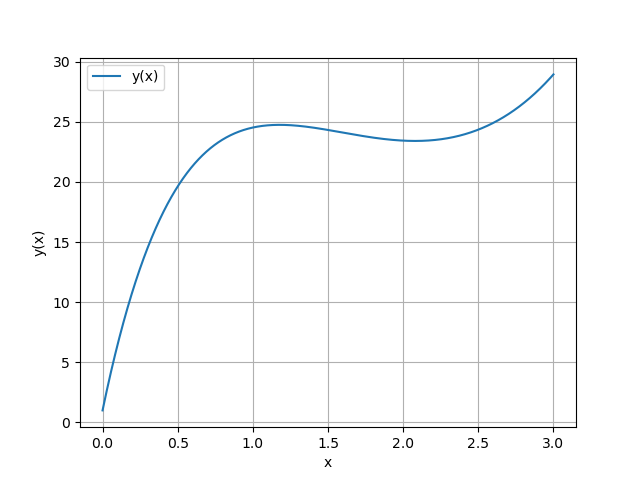
\includegraphics[width=1\linewidth]{2021/CE/26/figures/figure1.png}
        \caption{Plot of y(x)}
    \label{fig:enter-label}
\end{figure}


%\end{document}





\pagebreak
\item A system has a transfer function
\begin{align}
    G(s) = \frac{3e^{-4s}}{12s + 1}\nonumber
\end{align}
When a step-change of magnitude $M$ is given to the system input, the final value of the system output is measured to be 120. The value of M is \_\_\_\_\_.
\hfill(GATE 2021 CH Q52)\\
\solution
\iffalse
\let\negmedspace\undefined
\let\negthickspace\undefined
\documentclass[journal,12pt,twocolumn]{IEEEtran}
\usepackage{cite}
\usepackage{amsmath,amssymb,amsfonts,amsthm}
\usepackage{algorithmic}
\usepackage{graphicx}
\usepackage{textcomp}
\usepackage{xcolor}
\usepackage{txfonts}
\usepackage{listings}
\usepackage{enumitem}
\usepackage{mathtools}
\usepackage{gensymb}
\usepackage{comment}
\usepackage[breaklinks=true]{hyperref}
\usepackage{tkz-euclide} 
\usepackage{listings}
\usepackage{gvv}                            \usepackage{tikz}
\usepackage{circuitikz}
\def\inputGnumericTable{}                                
\usepackage[latin1]{inputenc}                            
\usepackage{color}                                       
\usepackage{array}                                       
\usepackage{longtable}                                   
\usepackage{calc}                              
\usepackage{tikz}
\usepackage{multirow}                                    
\usepackage{hhline}                                      
\usepackage{ifthen}                            
\usepackage{caption}
\usepackage{lscape}
\usepackage{amsmath}
\newtheorem{theorem}{Theorem}[section]
\newtheorem{problem}{Problem}
\newtheorem{proposition}{Proposition}[section]
\newtheorem{lemma}{Lemma}[section]
\newtheorem{corollary}[theorem]{Corollary}
\newtheorem{example}{Example}[section]
\newtheorem{definition}[problem]{Definition}
\newcommand{\BEQA}{\begin{eqnarray}}
\newcommand{\EEQA}{\end{eqnarray}}
\newcommand{\define}{\stackrel{\triangle}{=}}
\theoremstyle{remark}
\newtheorem{rem}{Remark}

\begin{document}

\bibliographystyle{IEEEtran}
\vspace{3cm}

\title{GATE 2021 CH Q52}
\author{EE23BTECH11009 - AROSHISH PRADHAN$^{*}$% <-this % stops a space
}
\maketitle
\newpage
\bigskip
\textbf{Question:} A system has a transfer function
\begin{align}
    G(s) = \frac{3e^{-4s}}{12s + 1}\nonumber
\end{align}
When a step-change of magnitude $M$ is given to the system input, the final value of the system output is measured to be 120. The value of M is \_\_\_\_\_.
\hfill(GATE 2021 CH Q52)\\
\solution
\fi
\begin{table}[!h]
    \centering
    \begin{tabular}{|c|c|c|}
    \hline
       \textbf{Symbol}  & \textbf{Value} & \textbf{Description}\\
    \hline
        $x(t)$ & $Mu(t)$ & Input Signal\\
    \hline
        $X(s)$ & $\frac{M}{s}$ & s-domain Input Signal\\
    \hline
        $y(t)$ &  & Output Signal\\
    \hline
        $Y(s)$ & & s-domain Output Signal\\
    \hline
       $G(s)$ & $\frac{3e^{-4s}}{12s + 1}$ & Transfer Function\\
    \hline
    \end{tabular}
    \caption{Given Parameters}
    \label{tab:1_gate.21.ch.52}
\end{table}


Given, input step-change:
\begin{align}
    x(t) &= Mu(t)\\
    u(t) &\system{L} \frac{1}{s}\\
    \implies X(s) &= \frac{M}{s}
\end{align}
Transfer Function:
\begin{align}
    G(s) &= \frac{Y(s)}{X(s)} = \frac{3e^{-4s}}{12s + 1}\\
    \implies Y(s) &= \frac{3e^{-4s}}{12s + 1}\frac{M}{s}
\end{align}
$\therefore$ system output
\begin{align}
     \lim_{s\rightarrow0}sY(s) &= 120\\
    \implies \lim_{s\rightarrow0}\brak{\frac{3e^{-4s}}{12s + 1}M} &= 120\\
    \implies 3M &= 120\\
    \implies M &= 40
\end{align}

\begin{figure}
    \centering
    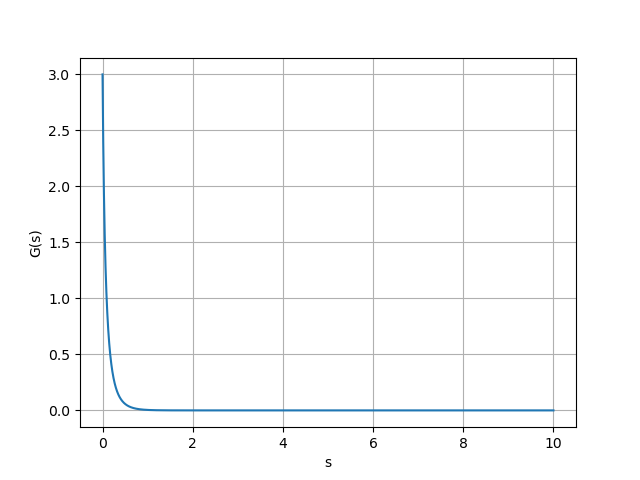
\includegraphics[width = \columnwidth]{2021/CH/52/figs/assign9.png}
	\caption{Plot of $G(s)$ vs $s$}
    \label{fig:1_gate.21.ch.52}
\end{figure}
%\end{document}

\pagebreak
\item The Bode magnitude plot for the transfer function $\frac{V_o(s)}{V_i(s)}$ of the circuit is as shown. The value of R is \_\_\_\_\_$\Omega$. \hfill(GATE 2021 EE Q20)
\begin{figure}[!ht]
    \centering
    \begin{circuitikz}
   \draw(0,0) to [R](2,0);
   % \draw (2,0) -- (2.5,0);
   \draw(2,0) to [L] (4,0);
   % \draw (5,0) to (5,0);
   \draw (4,0) to [C] (4,-2);
   \draw(4,-2)  to (0,-2);
   \draw (4,0) -- (5,0);
   \draw (4,-2)to (5,-2);
   \node[circle,fill,inner sep=1pt] at (0,0) {};
   \node[circle,fill,inner sep=1pt] at (5,0) {};
   \node[circle,fill,inner sep=1pt] at (5,-2) {};
   \node[circle,fill,inner sep=1pt] at (0,-2) {};
   \draw[->](0,-1.85) to (0,-0.15);
   \draw[->](5,-1.85) to (5,-0.15);
   \node at (0.3,-1) {$V_i$};
   \node at (5.5,-1) {$V_o$};

   \node at (1,0.5) {$R$};
   \node at (3,0.5) {$1mH$};
   \node at (2.8,-1) {$250\micro F$};\node[circle,fill,inner sep=1pt] at (0,0) {};
\end{circuitikz}

\end{figure}
\begin{figure}[!ht]
    \centering
    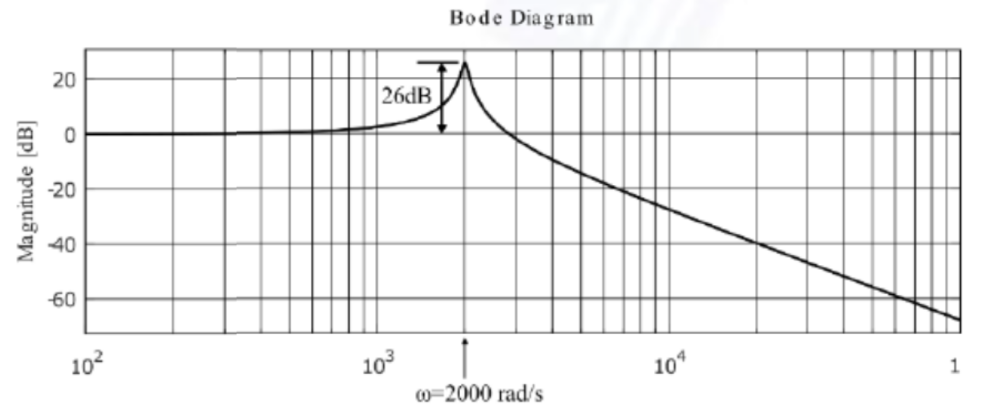
\includegraphics[width=\columnwidth]{2021/EE/20/figs/bode.png}
\end{figure}
\solution
\iffalse
\let\negmedspace\undefined
\let\negthickspace\undefined
\documentclass[journal,12pt,twocolumn]{IEEEtran}
\usepackage{cite}
\usepackage{amsmath,amssymb,amsfonts,amsthm}
\usepackage{algorithmic}
\usepackage{textcomp}
\usepackage{xcolor}
\usepackage{txfonts}
\usepackage{listings}
\usepackage{enumitem}
\usepackage{mathtools}
\usepackage{gensymb}
\usepackage{comment}
\usepackage[breaklinks=true]{hyperref}
\usepackage{tkz-euclide} 
\usepackage{listings}
\usepackage{gvv}                            \usepackage{tikz}
\usepackage{circuitikz}
\def\inputGnumericTable{}                                
\usepackage[latin1]{inputenc}                            
\usepackage{color}                                       
\usepackage{array}                                       
\usepackage{longtable}                                   
\usepackage{calc}                              
\usepackage{tikz}
\usepackage{multirow}                                    
\usepackage{hhline}                                      
\usepackage{ifthen}                            
\usepackage{caption}
\usepackage{lscape}
\usepackage{amsmath}
\newtheorem{theorem}{Theorem}[section]
\newtheorem{problem}{Problem}
\newtheorem{proposition}{Proposition}[section]
\newtheorem{lemma}{Lemma}[section]
\newtheorem{corollary}[theorem]{Corollary}
\newtheorem{example}{Example}[section]
\newtheorem{definition}[problem]{Definition}
\newcommand{\BEQA}{\begin{eqnarray}}
\newcommand{\EEQA}{\end{eqnarray}}
\newcommand{\define}{\stackrel{\triangle}{=}}
\theoremstyle{remark}
\newtheorem{rem}{Remark}

\begin{document}

\bibliographystyle{IEEEtran}
\vspace{3cm}

\title{GATE 2021 EE.20}
\author{EE23BTECH11010 - VENKATESH BANDAWAR$^{*}$% <-this % stops a space
}
\maketitle
\newpage
\bigskip
\textbf{Question:} The Bode magnitude plot for the transfer function $\frac{V_o(s)}{V_i(s)}$ of the circuit is as shown. The value of R is \_\_\_\_\_$\Omega$. \hfill(GATE 2021 EE Q20)
\begin{figure}[!ht]
    \centering
    \begin{circuitikz}
   \draw(0,0) to [R](2,0);
   % \draw (2,0) -- (2.5,0);
   \draw(2,0) to [L] (4,0);
   % \draw (5,0) to (5,0);
   \draw (4,0) to [C] (4,-2);
   \draw(4,-2)  to (0,-2);
   \draw (4,0) -- (5,0);
   \draw (4,-2)to (5,-2);
   \node[circle,fill,inner sep=1pt] at (0,0) {};
   \node[circle,fill,inner sep=1pt] at (5,0) {};
   \node[circle,fill,inner sep=1pt] at (5,-2) {};
   \node[circle,fill,inner sep=1pt] at (0,-2) {};
   \draw[->](0,-1.85) to (0,-0.15);
   \draw[->](5,-1.85) to (5,-0.15);
   \node at (0.3,-1) {$V_i$};
   \node at (5.5,-1) {$V_o$};

   \node at (1,0.5) {$R$};
   \node at (3,0.5) {$1mH$};
   \node at (2.8,-1) {$250\micro F$};\node[circle,fill,inner sep=1pt] at (0,0) {};
\end{circuitikz}

\end{figure}
\begin{figure}[!ht]
    \centering
    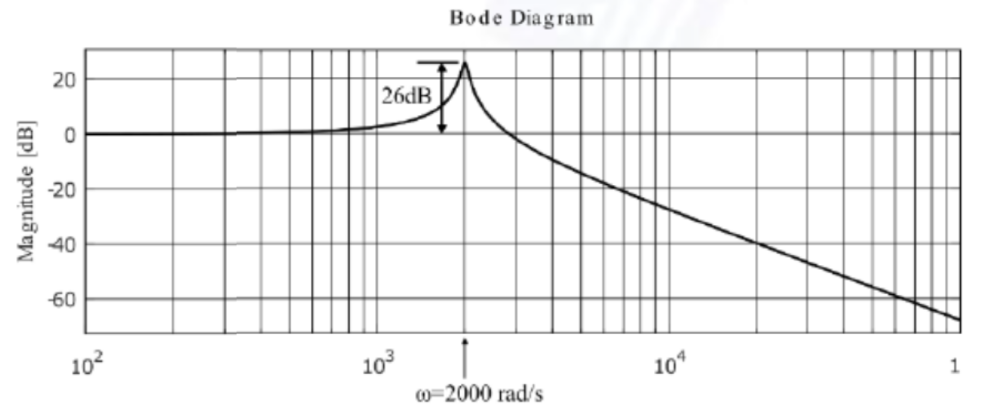
\includegraphics[width=\columnwidth]{2021/EE/20/figs/bode.png}
\end{figure}
\solution
\fi
\begin{table}[!ht]
    \centering
    \begin{tabular}{|c|c|c|}
\hline
    \textbf{Parameter} & \textbf{Description} & \textbf{Value} \\
    \hline
    $C$ & Capacitance & $250\micro F$\\
    \hline
    $L$ & Inductor & $1mH$\\
    \hline
    $I$ & Current &  \\
    \hline
    $I(0)$ & Initial Current & 0A \\
    \hline
    $V_o$ & Voltage across capacitor & \\
    \hline 
    $V_i$ & Input Voltage & \\
    \hline 
    $T(s)$ & Transfer Function & $\frac{V_o(s)}{V_i(s)}$\\
    \hline
    \end{tabular}

    \caption{Given Parameters table}
    \label{Given Parameters table_2021_EE_20}
\end{table}
Applying KVL,
\begin{align}
    V_i - R I - L\frac{dI}{dt} - \frac{\int I dt}{C} = 0
\end{align}
Taking Laplace Transform ,
\begin{align}
    V_i(s) &- RI(s) - LsI(s) + LI(0^+) - \frac{I(s)}{sC} = 0\\
    I(s) &= \frac{V_i(s) + LI(0)}{R + sL + \frac{1}{sC}}\\
    V_o(s) &= \frac{V_i(s) + LI(0)}{RsC + s^2LC + 1}
\end{align}
Substituting $I(0) = 0$ and $s = j\omega$,
\begin{align}
    \frac{V_o(j\omega)}{V_i(j\omega)} &= \frac{1}{\omega RCj -\omega^2LC + 1} 
\end{align}
$\because$ Magnitude in bode plot = $20\log \abs{T(s)}$\\
From given graph,At $\omega = 2000$
\begin{align}
    26 &= 20 \log \abs{\frac{V_o}{V_i}}\\
    \abs{\frac{V_o}{V_i}} &= 20
\end{align}
\begin{align}
    \implies 20 &= \abs{\frac{1}{\omega RCj -\omega^2LC + 1}} \\
    R &= 0.1 \Omega
\end{align}
\begin{figure}[!h]
    \centering
    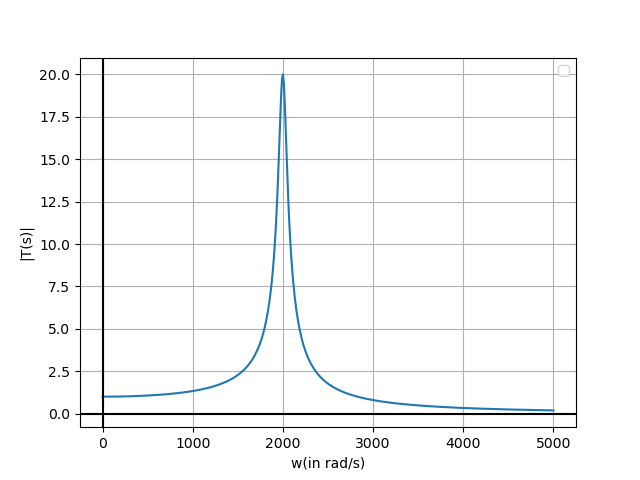
\includegraphics[width=\columnwidth]{2021/EE/20/figs/frequency_response.png}
    \caption{Frequency response of $V_o$}
    \label{frequency_response_2021_EE_20}
\end{figure}
%\end{document}

\pagebreak
\item Consider a system with transfer-function $G\brak{s}=\frac{2}{s+1}$. A unit-step function $\mu\brak{t}$ is applied to the system, which results in an output y\brak{t}. 

If $e\brak{t}=y\brak{t}-\mu\brak{t}$ then $ \lim_{t\to\infty} e(t)$ is\rule{1.5cm}{0.15mm}.
\solution
\iffalse
\let\negmedspace\undefined
\let\negthickspace\undefined
\documentclass[journal,12pt,twocolumn]{IEEEtran}
\usepackage{cite}
\usepackage{amsmath,amssymb,amsfonts,amsthm}
\usepackage{algorithmic}
\usepackage{graphicx}
\usepackage{textcomp}
\usepackage{xcolor}
\usepackage{txfonts}
\usepackage{listings}
\usepackage{enumitem}
\usepackage{mathtools}
\usepackage{gensymb}
\usepackage{comment}
\usepackage[breaklinks=true]{hyperref}
\usepackage{tkz-euclide} 
\usepackage{listings}
\usepackage{gvv}                                        
\def\inputGnumericTable{}                                 
\usepackage[latin1]{inputenc}                                
\usepackage{color}                                            
\usepackage{array}                                            
\usepackage{longtable}                                       
\usepackage{calc}                                             
\usepackage{multirow}                                         
\usepackage{hhline}                                           
\usepackage{ifthen}                                           
\usepackage{lscape}
\newtheorem{theorem}{Theorem}[section]
\newtheorem{problem}{Problem}
\newtheorem{proposition}{Proposition}[section]
\newtheorem{lemma}{Lemma}[section]
\newtheorem{corollary}[theorem]{Corollary}
\newtheorem{example}{Example}[section]
\newtheorem{definition}[problem]{Definition}
\newcommand{\BEQA}{\begin{eqnarray}}
\newcommand{\EEQA}{\end{eqnarray}}
\newcommand{\define}{\stackrel{\triangle}{=}}
\theoremstyle{remark}
\usepackage{circuitikz}
\newtheorem{rem}{Remark}
\begin{document}
\parindent 0px

\bibliographystyle{IEEEtran}
\vspace{3cm}

\title{Assignment\\[1ex]GATE-IN-46}
\author{EE23BTECH11034 - Prabhat Kukunuri$^{}$% <-this % stops a space
}
\maketitle
\newpage
\bigskip

\renewcommand{\thefigure}{\theenumi}
\renewcommand{\thetable}{\theenumi}
\section{Question}
Consider a system with transfer-function $G\brak{s}=\frac{2}{s+1}$. A unit-step function $\mu\brak{t}$ is applied to the system, which results in an output y\brak{t}. 

If $e\brak{t}=y\brak{t}-\mu\brak{t}$ then $ \lim_{t\to\infty} e(t)$ is\rule{1.5cm}{0.15mm}.

\solution
\fi
\begin{table}[h]
    \centering
    \begin{tabular}{|p{1cm}|p{3.00cm}|p{3.50cm}|}
    \hline
    Symbol&Value&Description\\ \hline
    $$G\brak{s}$$&$$\frac{2}{s+1}$$&$$\text{Transfer function}$$\\\hline
    $$e\brak{t}$$&$$y\brak{t}-\mu\brak{t}$$&$$\text{Function of y\brak{t} and $\mu\brak{t}$}$$\\\hline
    $$Y\brak{s}$$&$$G\brak{s}\times U\brak{s}$$&Convolution in $t$ domain is multiplication in $s$ domain.\\\hline
    $$\mu\brak{t}$$&$$\begin{cases}
    0&\text{if t$<$0}\\
    1&\text{if t$>$0}
    \end{cases}$$&$$\text{Unit step function}$$\\\hline
    \end{tabular}
    \caption{Variable description}
    \label{tab:GATE.2021.IN.46.1}
\end{table}\\
Applying Laplace transform on $\mu\brak{t}$
\begin{align}
    &\mu\brak{t}\system{L}U\brak{s}\\
    &U\brak{s}=\frac{1}{s}\\
    &Y\brak{s}=\brak{\frac{2}{s+1}}\brak{\frac{1}{s}}\\
    &Y\brak{s}=\frac{2}{s}-\frac{2}{s+1}
\end{align}
The inverse Laplace transform of $\frac{a}{s+b}$ is $ae^{-bt}\mu\brak{t}$
\begin{align}
    &y\brak{t}=2\mu\brak{t}-2e^{-t}\mu\brak{t}\\
    &e\brak{t}=\mu\brak{t}\brak{1-2e^{-t}}\\
    &\lim_{t\to\infty}e\brak{t}=\lim_{t\to\infty}\mu\brak{t}\brak{1-2e^{-t}}\\
    &\lim_{t\to\infty}e\brak{t}=1
\end{align}
%\end{document}

\end{enumerate}

 \section{2021}
\chapter{Fourier transform}
\section{2021}
 \begin{enumerate}[label=\thechapter.\arabic*,ref=\thechapter.\theenumi]
\item Consider the signals $x\brak{n}$=$2^{n-1} u\brak{ -n+2}$ and $y\brak{n}$=$2^{-n+2}u\brak{ n+1}$, where $u\brak{n}$ is the unit step sequence. Let $X\brak{e^{j\omega}}$ and $Y\brak{e^{j\omega}}$ be the discrete-time Fourier of $x\brak{n}$ and $y\brak{n}$,respectively. The value of the integral $\frac{1}{2\pi}\int_{0}^{2\pi} X\brak{e^{j\omega}} Y\brak{e^{-j\omega}} d \omega$
(rounded off to one decimal place) is \underline{{\hspace{1.5in}}}\\
\hfill{(GATE EC 41 2021)}\\
\solution

\let\negmedspace\undefined
\let\negthickspace\undefined
\documentclass[journal,12pt,twocolumn]{IEEEtran}
\usepackage{cite}
\usepackage{amsmath,amssymb,amsfonts,amsthm}
\usepackage{algorithmic}
\usepackage{graphicx}
\usepackage{textcomp}
\usepackage{xcolor}
\usepackage{txfonts}
\usepackage{listings}
\usepackage{enumitem}
\usepackage{mathtools}
\usepackage{gensymb}
\usepackage{comment}
\usepackage[breaklinks=true]{hyperref}
\usepackage{tkz-euclide} 
\usepackage{listings}
\usepackage{gvv}                                        
\def\inputGnumericTable{}                                 
\usepackage[latin1]{inputenc}                                
\usepackage{color}                                            
\usepackage{array}                                            
\usepackage{longtable}                                       
\usepackage{calc}                                             
\usepackage{multirow}                                         
\usepackage{hhline}                                           
\usepackage{ifthen}                                           
\usepackage{lscape}

\newtheorem{theorem}{Theorem}[section]
\newtheorem{problem}{Problem}
\newtheorem{proposition}{Proposition}[section]
\newtheorem{lemma}{Lemma}[section]
\newtheorem{corollary}[theorem]{Corollary}
\newtheorem{example}{Example}[section]
\newtheorem{definition}[problem]{Definition}
\newcommand{\BEQA}{\begin{eqnarray}}
\newcommand{\EEQA}{\end{eqnarray}}
\newcommand{\define}{\stackrel{\triangle}{=}}
\theoremstyle{remark}
\newtheorem{rem}{Remark}
\begin{document}
\bibliographystyle{IEEEtran}
\vspace{3cm}
\title{\textbf{EC-2021}}
\author{EE23BTECH11210-Dhyana Teja Machineni$^{*}$% <-this % stops a space
}
\maketitle
\newpage
\bigskip

\textbf{QUESTION:}\\
Consider the signals $x\brak{n}$=$2^{n-1} u\brak{ -n+2}$ and $y\brak{n}$=$2^{-n+2}u\brak{ n+1}$, where $u\brak{n}$ is the unit step sequence. Let $X\brak{e^{j\omega}}$ and $Y\brak{e^{j\omega}}$ be the discrete-time Fourier of $x\brak{n}$ and $y\brak{n}$,respectively. The value of the integral $\frac{1}{2\pi}\int_{0}^{2\pi} X\brak{e^{j\omega}} Y\brak{e^{-j\omega}} d \omega$
(rounded off to one decimal place) is \underline{{\hspace{1.5in}}}\\
\hfill{(GATE EC 41 2021)}\\

\solution\\

\begin{table}[h]
         
\begin{tabular}{|c|c|l|}
\hline
Parameter  & Value & Description   \\             
\hline
$y(0)$     & $0$   & Initial displacement  \\     
 \hline
$y'(0)$    & $0$   & First derivative at $t=0$  \\
 \hline
$y''(0)$   & $0$   & Second derivative at $t=0$ \\
 \hline
$y'''(0)$  & $0$   & Third derivative at $t=0$  \\
 \hline
\end{tabular}


         \caption{Variables and their descriptions}
     \end{table}
\begin{align}
    V&=\frac{1}{2\pi}\int_{0}^{2\pi} X\brak{e^{j\omega}} Y\brak{e^{-j\omega}} d \omega\\
     Z\brak{e^{j\omega}}&= X\brak{e^{j\omega}} Y\brak{e^{-j \omega}}\\
           z(n)&\xrightarrow{\mathcal{F}} Z(e^{j\omega})\\
           z\brak{n}&=\frac{1}{2\pi}\int_{-\pi}^{\pi} Z\brak{e^{j\omega}} e^{j\omega n} d\omega\\
      z\brak{0}&=\frac{1}{2\pi}\int_{0}^{2\pi} Z\brak{e^{j\omega}} d \omega\\
   z\brak{ n}&= x\brak{n} * y\brak{-n}\\
   &=\sum_{k=-\infty}^{\infty} 2^{k-1} u\brak{-k+2} 2^{n-k+2} u\brak{-n+k+1}\\
   &=\sum_{k=-\infty}^{2} 2^{n+1} u\brak{k-n+1}\\
   z(0)&=\sum_{k=-\infty}^{2} 2 u\brak{k+1}\\
   &=2\sum_{k=-1}^{2}u\brak{k+1}\\
  \therefore z\brak{0} &=8
\end{align}
$\therefore$ $\frac{1}{2\pi}\int_{0}^{2\pi} X\brak{e^{j\omega}} Y\brak{e^{-j\omega}} d \omega$= $8$
\renewcommand{\thefigure}{\theenumi}
 \renewcommand{\thetable}{\theenumi}
\begin{figure}[h]
  
  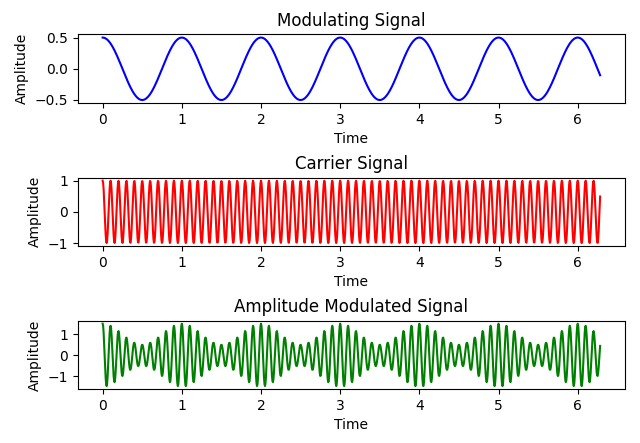
\includegraphics[width=\columnwidth]{figs/Figure_1.png}
  \caption{Stem Plot of $z\brak{n}$}
\end{figure}
\end{document}

\pagebreak
\item Given that $\mathcal{S}$ is the unit circle in the counter clock-wise direction with its centre at origin, the integral
        $\oint \brak{\frac{z^3}{4z-\jmath}}dz=\rule{1cm}{0.15mm}$
 (round off to theree decimal places)
 \hfill{(GATE 2022 AE)}\\
 \solution\\
 


\item Consider the signals \(x[n] = 2^{n-1} u[-n+2]\) and \(y[n] = 2^{-n+2} u[n+1]\), where \(u[n]\) is the unit step sequence. Let \(X(e^{j\omega})\) and \(Y(e^{j\omega})\) be the discrete-time Fourier transform of \(x[n]\) and \(y[n]\), respectively. The value of the integral
\[
\frac{1}{2\pi} \int_{0}^{2\pi} X(e^{j\omega}) Y(e^{-j\omega}) d\omega
\]
(rounded off to one decimal place) is.\\
\hfill{GATE 2021 EC 41 Q}
\solution
\iffalse
\let\negmedspace\undefined
\let\negthickspace\undefined
\documentclass[journal,12pt,twocolumn]{IEEEtran}
\usepackage{pgfplots}
\pgfplotsset{compat=1.17}
\usepackage{cite}
\usepackage{amsmath,amssymb,amsfonts,amsthm}
\usepackage{algorithmic}
\usepackage{graphicx}
\usepackage{textcomp}
\usepackage{xcolor}
\usepackage{txfonts}
\usepackage{listings}
\usepackage{enumitem}
\usepackage{mathtools}
\usepackage{gensymb}
\usepackage{comment}
\usepackage[breaklinks=true]{hyperref}
\usepackage{tkz-euclide} 
\usepackage{listings}
\usepackage{gvv}                                        
\def\inputGnumericTable{}                                 
\usepackage[latin1]{inputenc}                                
\usepackage{color}                                            
\usepackage{array}                                            
\usepackage{longtable}                                       
\usepackage{calc}                                             
\usepackage{multirow}                                         
\usepackage{hhline}                                           
\usepackage{ifthen}                                           
\usepackage{lscape}
\newtheorem{theorem}{Theorem}[section]
\newtheorem{problem}{Problem}
\newtheorem{proposition}{Proposition}[section]
\newtheorem{lemma}{Lemma}[section]
\newtheorem{corollary}[theorem]{Corollary}
\newtheorem{example}{Example}[section]
\newtheorem{definition}[problem]{Definition}
\newcommand{\BEQA}{\begin{eqnarray}}
\newcommand{\EEQA}{\end{eqnarray}}
\newcommand{\define}{\stackrel{\triangle}{=}}
\theoremstyle{remark}
\newtheorem{rem}{Remark}
\begin{document}
\bibliographystyle{IEEEtran}
\vspace{3cm}
\title{GATE EC 41Q}
\author{EE23BTECH11021 - GANNE GOPI CHANDU$^{*}$% <-this % stops a space
}
\maketitle
\bigskip
\renewcommand{\thefigure}{\theenumi}
\renewcommand{\thetable}{\theenumi}
\bibliographystyle{IEEEtran}
\textbf{Question}\\
Consider the signals \(x[n] = 2^{n-1} u[-n+2]\) and \(y[n] = 2^{-n+2} u[n+1]\), where \(u[n]\) is the unit step sequence. Let \(X(e^{j\omega})\) and \(Y(e^{j\omega})\) be the discrete-time Fourier transform of \(x[n]\) and \(y[n]\), respectively. The value of the integral
\[
\frac{1}{2\pi} \int_{0}^{2\pi} X(e^{j\omega}) Y(e^{-j\omega}) d\omega
\]
(rounded off to one decimal place) is.\\
\textbf{Solution}\\
\fi
\begin{table}[!h]
\begin{center}
\renewcommand\thetable{1}
\begin{tabular}{ |c|c|c| } 
  \hline
    Symbol & Value & description \\ 
  \hline
  $x[n] $ & $2^{n-1}u[-n+2]$ & Discrete time signal  \\ 
  \hline
  $y[n] $ & $2^{-n+2}u[n+1]$ & Discrete time signal  \\ 
  \hline
\end{tabular}
\end{center}
\caption{}
\end{table}
\begin{align}
     x[n]*y[n] && \xleftrightarrow[transform]{Fourier} && X(e^{j\omega}) Y(e^{j\omega})\\
 x[n] && \xleftrightarrow [transform]{Fourier} && X(e^{j\omega}) \\
 y[n] && \xleftrightarrow [transform]{Fourier} && Y(e^{j\omega}) 
\end{align}
The
 \begin{align}
       y(n) && \xleftrightarrow [transform]{Fourier} && y(e^{j\omega})
\end{align}
By using the time reversal property:
\begin{align}
y[-n] && \xleftrightarrow [transform]{Fourier} && y(e^{-j\omega})
\end{align}
Let assume
\begin{align}
     z[n]& = x[n] * y[-n]\\
     Z\brak{e^{j \omega}} &=X(e^{j\omega}) Y(e^{-j\omega})
 \end{align}
\begin{align}
      z[n]& =\frac{1}{2\pi} \int_{0}^{2\pi} Z(e^{j\omega})e^{j \omega n} d\omega \\
      &=\frac{1}{2\pi} \int_{0}^{2\pi}  X(e^{j\omega}) Y(e^{-j\omega})e^{j \omega n} d\omega.
 \end{align}
 putting  n=0, we get
\begin{align}
    z[0]&=\frac{1}{2\pi} \int_{0}^{2\pi} X(e^{j\omega}) Y(e^{-j\omega}) d\omega
\end{align}
\begin{align}
    z[n] = x[n] * y[-n]\\
 &= \sum_{k=-\infty}^{\infty} 2^{k-1} u[-k+2]\cdot 2^{n-k+2} u[-n+k+1]\\
 &= \sum_{k=-\infty}^{2} 2^{k-1} \cdot 2^{n-k+2} u[-n+k+1]\\
 &= \sum_{k=-\infty}^{2} 2^{k-1+n-k+2} u[-n+k+1]\\
 &= \sum_{k=-\infty}^{2} 2^{n+1} u[-n+k+1]
\end{align}

Putting $n = 0$, we get:
\begin{align}
     \frac{1}{2\pi} \int_{0}^{2\pi} X(e^{j\omega}) Y(e^{-j\omega}) d\omega &= z[0]\\
     &= \sum_{k=-\infty}^{2} 2 \cdot u[k+1] \\
     &=\sum_{k=-1}^{2} 2(1) = 2 \times 4 \\
     &= 8
\end{align}

\pagebreak
\item Consider a continuous-time signal $x\brak{t}$ \,defined by $x\brak{t}=0$\,for $\abs{t}>1$, and $x\brak{t}=1-\abs{t}$ for $\abs{t}\le 1$. Let the Fourier transform of $x\brak{t}$ be defined as $X\brak{\omega}=\int_{-\infty}^{\infty}x\brak{t}e^{-j\omega t} dt$. The maximum magnitude of $X\brak{\omega}$ is $\hbox to 4em{\thinspace\hrulefill\thinspace}$.
\hfill{(GATE 2021 EE 43)}\\
\solution
%\iffalse
\let\negmedspace\undefined
\let\negthickspace\undefined
\documentclass[journal,12pt,onecolumn]{IEEEtran}
\usepackage{cite}
\usepackage{amsmath,amssymb,amsfonts,amsthm}
\usepackage{algorithmic}
\usepackage{graphicx}
\usepackage{textcomp}
\usepackage{xcolor}
\usepackage{txfonts}
\usepackage{listings}
\usepackage{enumitem}
\usepackage{mathtools}
\usepackage{gensymb}
\usepackage{comment}
\usepackage{caption}
\usepackage[breaklinks=true]{hyperref}
\usepackage{tkz-euclide} 
\usepackage{listings}
\usepackage{gvv}                                        
\def\inputGnumericTable{}                                 
\usepackage[latin1]{inputenc}                                
\usepackage{color}                                            
\usepackage{array}                                            
\usepackage{longtable}                                       
\usepackage{calc}                                             
\usepackage{multirow}                                         
\usepackage{hhline}                                           
\usepackage{ifthen}                                           
\usepackage{lscape}

\newtheorem{theorem}{Theorem}[section]
\newtheorem{problem}{Problem}
\newtheorem{proposition}{Proposition}[section]
\newtheorem{lemma}{Lemma}[section]
\newtheorem{corollary}[theorem]{Corollary}
\newtheorem{example}{Example}[section]
\newtheorem{definition}[problem]{Definition}
\newcommand{\BEQA}{\begin{eqnarray}}
\newcommand{\EEQA}{\end{eqnarray}}
\newcommand{\define}{\stackrel{\triangle}{=}}
\theoremstyle{remark}
\newtheorem{rem}{Remark}
\begin{document}

\bibliographystyle{IEEEtran}
\vspace{3cm}

\title{GATE 2021 EE 43}
\author{EE23BTECH11022 - G DILIP REDDY}
\maketitle

\bigskip

\renewcommand{\thefigure}{\arabic{figure}}
\renewcommand{\thetable}{\arabic{table}}
\textbf{Question}:\\
Consider a continuous-time signal $x\brak{t}$ \,defined by $x\brak{t}=0$\,for $\abs{t}>1$, and $x\brak{t}=1-\abs{t}$ for $\abs{t}\le 1$. Let the Fourier transform of $x\brak{t}$ be defined as $X\brak{\omega}=\int_{-\infty}^{\infty}x\brak{t}e^{-j\omega t} dt$. The maximum magnitude of $X\brak{\omega}$ is $\hbox to 4em{\thinspace\hrulefill\thinspace}$.
\hfill{(GATE 2021 EE 43)}
\\\\
\solution
%\fi
\begin{align}
X\brak{f}&=\int_{-\infty}^{\infty}x\brak{t}e^{-j2\pi f t} dt\\
X\brak{f}&=\int_{-1}^{1}\brak{1-\abs{t}}e^{-j2\pi f t} dt\\
X\brak{f}&=\int_{-1}^{1}e^{-j2\pi f t} 
dt - \int_{-1}^{1}\abs{t}e^{-j2\pi f t} dt\\
X\brak{f}&=2\int_{0}^{1}\cos\brak{{2\pi f t}}
dt - 2\int_{0}^{1}t\cos\brak{2\pi f t} dt\\
X\brak{f}&=2\frac{\sin\brak{{2\pi f }}}{2\pi f}
- 2\sbrak{\frac{\sin\brak{2\pi f }}{2\pi f}+\frac{\cos\brak{2\pi f }}{\brak{2\pi f}^2}-\frac{1}{\brak{2\pi f }^2}}\\
X\brak{f}&=2\frac{1-\cos\brak{2\pi f }}{\brak{2\pi f}^2}\\
X\brak{f}&=2\frac{2\sin^2\brak{\frac{2\pi f}{2}}}{\brak{2\pi f}^2}\\
X\brak{f}&=\frac{\sin^2\brak{\pi f}}{\brak{\pi f}^2}\\
f& \to 0 \implies X\brak{f}\to1
\end{align}
Maximum of magnitude of $X\brak{f}=1$
\begin{figure}[h]
    \centering
    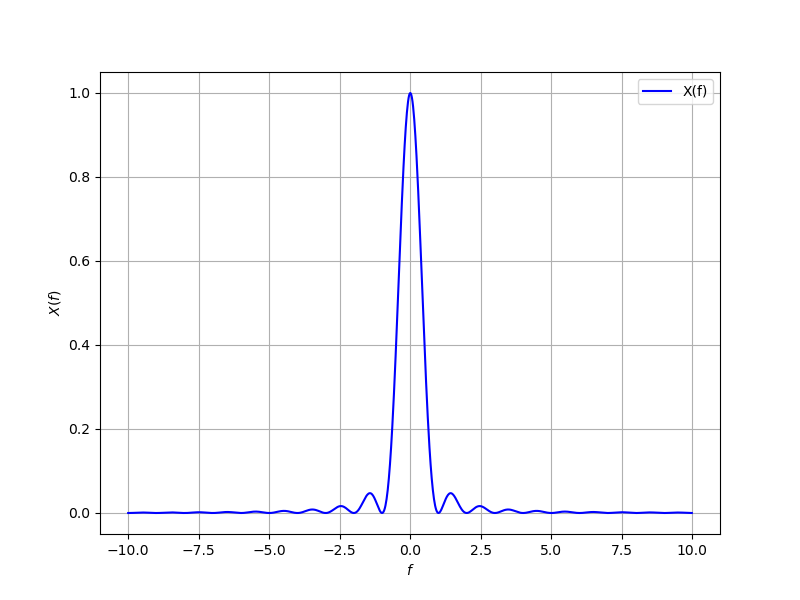
\includegraphics[width=1\linewidth]{figs/graph.png}
    \caption{plot of X(f)}
\end{figure}
\end{document}
\pagebreak
\item Let $f(t)$ be an even function, i.e.$f(-t) = f(t)$ for all t.Let the Fourier transform of $f(t)$ be defined as $F(\omega) = \int_{-\infty}^{\infty} f(t) e^{-j \omega t} \, dt $ . Suppose $\dfrac{dF(\omega)}{d \omega} = -\omega F(\omega)$ for all $\omega$ , and $F(0) = 1$ . Then


\begin{enumerate}[label = (\Alph*)]
\item $f(0) < 1 $\\
\item  $f(0) > 1 $\\
\item  $f(0) = 1 $\\
\item   $f(0) = 0 $\\
\end{enumerate} \hfill{(GATE EE 2021)}\\
\solution
\let\negmedspace\undefined
\let\negthickspace\undefined
\documentclass[journal,12pt,twocolumn]{IEEEtran}
\usepackage{cite}
\usepackage{amsmath,amssymb,amsfonts,amsthm}
\usepackage{algorithmic}
\usepackage{graphicx}
\usepackage{textcomp}
\usepackage{xcolor}
\usepackage{txfonts}
\usepackage{listings}
\usepackage{enumitem}
\usepackage{mathtools}
\usepackage{gensymb}
\usepackage{comment}
\usepackage[breaklinks=true]{hyperref}
\usepackage{tkz-euclide} 
\usepackage{listings}
\usepackage{gvv}  
\usepackage{tikz}
\usepackage{circuitikz} 
\usepackage{caption}
\def\inputGnumericTable{}              
\usepackage[latin1]{inputenc}          
\usepackage{color}                    
\usepackage{array}                     
\usepackage{longtable}                 
\usepackage{calc}                     \usepackage{multirow}                  
\usepackage{hhline}                    
\usepackage{ifthen}                    
\usepackage{lscape}
\usepackage{amsmath}
\newtheorem{theorem}{Theorem}[section]
\newtheorem{problem}{Problem}
\newtheorem{proposition}{Proposition}[section]
\newtheorem{lemma}{Lemma}[section]
\newtheorem{corollary}[theorem]{Corollary}
\newtheorem{example}{Example}[section]
\newtheorem{definition}[problem]{Definition}
\newcommand{\BEQA}{\begin{eqnarray}}
\newcommand{\EEQA}{\end{eqnarray}}
\newcommand{\define}{\stackrel{\triangle}{=}}
\theoremstyle{remark}
\newtheorem{rem}{Remark}

%\bibliographystyle{ieeetr}
\begin{document}
%

\bibliographystyle{IEEEtran}




\title{
%	\logo{
G.A.T.E.

\large{EE1205 : Signals and Systems}

Indian Institute of Technology Hyderabad
%	}
}
\author{Chirag Garg

(EE23BTECH11206)
}	





\maketitle

\newpage



\bigskip

\renewcommand{\thefigure}{\theenumi}
\renewcommand{\thetable}{\theenumi}


\section{Question E.E.(32)}
\vspace{0.5cm}



\textbf{Question:} 
Let $f(t)$ be an even function, i.e.$f(-t) = f(t)$ for all t.Let the Fourier transform of $f(t)$ be defined as $F(\omega) = \int_{-\infty}^{\infty} f(t) e^{-j \omega t} \, dt $ . Suppose $\dfrac{dF(\omega)}{d \omega} = -\omega F(\omega)$ for all $\omega$ , and $F(0) = 1$ . Then


\begin{enumerate}[label = (\Alph*)]
\item $f(0) < 1 $\\
\item  $f(0) > 1 $\\
\item  $f(0) = 1 $\\
\item   $f(0) = 0 $\\
\end{enumerate} \hfill{(GATE EE 2021)}\\
%\section{Solution} 
\textbf{Solution: }
Given, \begin{align}
\dfrac{dF(\omega)}{d \omega} &= -\omega F(\omega) \\
\dfrac{dF(\omega)}{d \omega} + \omega F(\omega) &= 0 \\
ln|F(\omega)| &= -\dfrac{\omega^{2}}{2} + c \\
F(\omega) &= Ke^{-\frac{\omega^2}{2}}
\end{align}
Put $\omega = 0$ , \begin{align}
F(0) &= K \\
K&=1
\end{align}
\begin{align}
\therefore F(\omega) &= e^{-\frac{\omega^2}{2}}
\end{align}

\begin{center}
 $f(t) \longleftrightarrow F(\omega)$
\end{center}
 \begin{align}
e^{-at^{2}}  \longleftrightarrow  \sqrt{\dfrac{\pi}{a}}
e^{-\frac{\omega^2}{4a}} \; ; \; a > 0 \\
At \; a = \dfrac{1}{2} , \; e^{-\frac{t^{2}}{2}}  \longleftrightarrow  \sqrt{2\pi} e^{-\frac{\omega^2}{2}}\\
\dfrac{1}{\sqrt{2\pi}}e^{-\frac{t^{2}}{2}}  \longleftrightarrow  e^{-\frac{\omega^2}{2}} = F(\omega) \\
\text{Thus , } f(t) = \dfrac{1}{\sqrt{2\pi}}e^{-\frac{t^{2}}{2}} 
 \end{align}
 At $t = 0$  \begin{align}
 f(0) = \dfrac{1}{\sqrt{2\pi}} < 1
 \end{align}
 Hence , option (a) is correct.
\end{document}
\pagebreak
\item The exponential Fourier series representation of a continous-time periodic signal x\brak{t} is defined as\\
\begin{center}
$x\brak{t}=\sum\limits_{k=-\infty}^{\infty}a_ke^{jk\omega_0t}$\\
\end{center}
where $\omega_0$ is the fundamental angular frequency of x\brak{t} and the coefficients of the series are $a_k$.The following information is given about x\brak{t} and $a_k$\\
I. x\brak{t} is real and even,having a fundamental period of 6\\
II. The average value of x\brak{t} is 2.\\
III.\begin{align}
 a_k= \begin{cases} 
      k, & 1 \leq k \leq 3 \\
      0, &  k > 3 
   \end{cases}\\
   \end{align}
The average power of the signal x\brak{t} (rounded off to one decimal place) is \underline{\hspace{1cm}}. \\
\hfill(GATE EC 2021)\\
\solution\\
\iffalse
\let\negmedspace\undefined
\let\negthickspace\undefined
\documentclass[a4,12pt,onecolumn]{IEEEtran}
\usepackage{amsmath,amssymb,amsfonts,amsthm}
\usepackage{algorithmic}
\usepackage{graphicx}
\usepackage{textcomp}
\usepackage{xcolor}
\usepackage{txfonts}
\usepackage{listings}
\usepackage{enumitem}
\usepackage{mathtools}
\usepackage{gensymb}
\usepackage[breaklinks=true]{hyperref}
\usepackage{tkz-euclide}
\usepackage{listings}
\usepackage{circuitikz}
\usepackage{gvv}
\begin{document}
\title{
\Huge\textbf{ GATE 2021 Assignment}\\
\Huge\textbf{EE1205} Signals and Systems\\
}
\large\author{Kurre Vinay\\EE23BTECH11036}
\maketitle
\textbf{Question:}
The exponential Fourier series representation of a continous-time periodic signal x\brak{t} is defined as\\
\begin{center}
$x\brak{t}=\sum\limits_{k=-\infty}^{\infty}a_ke^{jk\omega_0t}$\\
\end{center}
where $\omega_0$ is the fundamental angular frequency of x\brak{t} and the coefficients of the series are $a_k$.The following information is given about x\brak{t} and $a_k$\\
I. x\brak{t} is real and even,having a fundamental period of 6\\
II. The average value of x\brak{t} is 2.\\
III.\begin{align}
 a_k= \begin{cases} 
      k, & 1 \leq k \leq 3 \\
      0, &  k > 3 
   \end{cases}\\
   \end{align}
The average power of the signal x\brak{t} (rounded off to one decimal place) is \underline{\hspace{1cm}}. \\
\hfill(GATE EC 2021)\\
\solution\\
\fi
\begin{table}[ht!]
\begin{center}
\begin{tabular}{|c|c|c|}
   \hline
   variable&value&description\\
   \hline
   $T_0$&6&Fundamental time period\\
   \hline
  $P_{avg}$&-&average power of the signal\\
   \hline
   x\brak{t}&$\sum\limits_{k=-\infty}^{\infty}a_ke^{jk\omega_0t}$&Input signal\\
   \hline
   $a_k$& $\begin{cases} 
      k, & 1 \leq k \leq 3 \\
      0, &  k > 3 
   \end{cases}$&coefficients of the series \\
   \hline
  $a_0$&2&average of x\brak{t}\\
   \hline
\end{tabular}
\caption{Table: Input Parameters}
\end{center}
\end{table}\\
x\brak{t} is even and real so, $a_k$=$a_{-k}$\\
Parswal's Power Theorem\\
Proof
\begin{align}
P&=\frac{1}{T}\int\limits_{\frac{-T}{2}}^{\frac{T}{2}}\left| x\brak{t}^2 \right|dt ,\quad{\left| x\brak{t}^2 \right|=x\brak{t}x^*\brak{t}}\\
P&=\frac{1}{T}\int\limits_{\frac{-T}{2}}^{\frac{T}{2}}x\brak{t}x^*\brak{t}dt \\
x\brak{t}&=\sum\limits_{n=-\infty}^{\infty}C_ne^{jn\omega_0t}\\
P&=\frac{1}{T}\int\limits_{\frac{-T}{2}}^{\frac{T}{2}}\brak{\sum\limits_{k=-\infty}^{\infty}C_ne^{jn\omega_0t}}x^*\brak{t}dt\\
P&=\sum\limits_{n=-\infty}^{\infty}C_n\brak{\frac{1}{T}\int\limits_{\frac{-T}{2}}^{\frac{T}{2}}x^*\brak{t}e^{jn\omega_0t}dt}\\
&=\sum\limits_{n=-\infty}^{\infty}C_nC^*_n\\
\implies P&=\sum\limits_{n=-\infty}^{\infty}\left| C_n \right|^2
\end{align}
By using Parsval's Power Theorem
\begin{align}
\frac{1}{T}\int\limits_{0}^{T}\left| x\brak{t}^2 \right|dt&=\sum\limits_{k=-\infty}^{\infty}\left| a_k \right|^2\\
P_{avg}&=\sum\limits_{k=-\infty}^{\infty}\left| a_k \right|^2\\
&=2\sum\limits_{k=1}^{\infty}\left| a_k \right|^2 +|a_0|^2\\
&=2\sum\limits_{k=1}^{3}\left| a_k \right|^2  +|a_0|^2 \\
&=2\brak{1^2+2^2+3^2}+2^2\\
&=32\\
x\brak{n}&=2\text{Re}\brak{e^{\frac{j\pi t}{3}}+2e^{\frac{2j\pi t}{3}}+3e^{j\pi t}} + 2\\
\implies x\brak{n}&=2\brak{cos\brak{\frac{\pi t}{3}}+2cos\brak{\frac{2\pi t}{3}}+3cos\brak{\pi t}} + 2
\end{align}
The average power of the signal x\brak{t} (rounded off to one decimal place) is $32$
\begin{figure}[ht!]
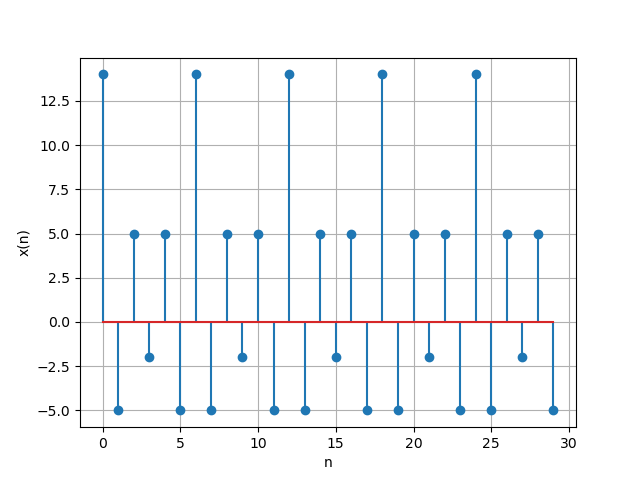
\includegraphics[width=\columnwidth]{2021/EC/39/figs/fig.png}
\caption{\large{STEM PLOT OF $y\brak{n}$}}
\end{figure}


\pagebreak
\item Let $X\brak{j \omega}$ denotes the Fourier transform of $x\brak{t}$. If 
\begin{align}
X\brak{j \omega} =& 10e^{-j\pi f \: \brak{\dfrac{sin\brak{\pi f}}{\pi f}}}
\end{align} 
then $ \dfrac{1}{2\pi} \int_{-\infty }^{\infty} X\brak{j \omega} d\omega = \rule{1cm}{0.15mm}$ .  (where $\omega$ = $2\pi f$)\\
\begin{enumerate}[label = \brak{\Alph*}]
\item 10$\pi$ \\
\item 100 \\
\item 10 \\
\item 20$\pi$ 
\end{enumerate}
\hfill GATE 2021\\
\solution
%\iffalse
\let\negmedspace\undefined
\let\negthickspace\undefined
\documentclass[journal,12pt,twocolumn]{IEEEtran}
\usepackage{cite}
\usepackage{amsmath,amssymb,amsfonts,amsthm}
\usepackage{algorithmic}
\usepackage{graphicx}
\usepackage{textcomp}
\usepackage{xcolor}
\usepackage{txfonts}
\usepackage{listings}
\usepackage{enumitem}
\usepackage{mathtools}
\usepackage{gensymb}
\usepackage{comment}
\usepackage[breaklinks=true]{hyperref}
\usepackage{tkz-euclide} 
\usepackage{listings}
\usepackage{gvv}  
\usepackage{tikz}
\usepackage{circuitikz} 
\usepackage{caption}

\def\inputGnumericTable{}                                
\usepackage[latin1]{inputenc}                 
\usepackage{color}                            
\usepackage{array}                            
\usepackage{longtable}                        
\usepackage{calc}                            
\usepackage{multirow}                      
\usepackage{hhline}                           
\usepackage{ifthen}                          
\usepackage{lscape}
\usepackage{amsmath}
\newtheorem{theorem}{Theorem}[section]
\newtheorem{problem}{Problem}
\newtheorem{proposition}{Proposition}[section]
\newtheorem{lemma}{Lemma}[section]
\newtheorem{corollary}[theorem]{Corollary}
\newtheorem{example}{Example}[section]
\newtheorem{definition}[problem]{Definition}
\newcommand{\BEQA}{\begin{eqnarray}}
\newcommand{\EEQA}{\end{eqnarray}}
\newcommand{\define}{\stackrel{\triangle}{=}}
\theoremstyle{remark}
\newtheorem{rem}{Remark}


\begin{document}
%

\bibliographystyle{IEEEtran}


\vspace{3cm}

\title{
%	\logo{
GATE 2021 BM

\large{EE:1205 Signals and System}

Indian Institute of Technology, Hyderabad
%	}
}
\author{Prashant Maurya

EE23BTECH11218
}	
%\title{
%	\logo{Matrix Analysis through Octave}{\begin{center}\includegraphics[scale=.24]{tlc}\end{center}}{}{HAMDSP}
%}


% paper title
% can use linebreaks \\ within to get better formatting as desired
%\title{Matrix Analysis through Octave}
%
%
% author names and IEEE memberships
% note positions of commas and nonbreaking spaces ( ~ ) LaTeX will not break
% a structure at a ~ so this keeps an author's name from being broken across
% two lines.
% use \thanks{} to gain access to the first footnote area
% a separate \thanks must be used for each paragraph as LaTeX2e's \thanks
% was not built to handle multiple paragraphs
%

%\author{<-this % stops a space
%\thanks{}}
%}
% note the % following the last \IEEEmembership and also \thanks - 
% these prevent an unwanted space from occurring between the last author name
% and the end of the author line. i.e., if you had this:
% 
% \author{....lastname \thanks{...} \thanks{...} }
%                     ^------------^------------^----Do not want these spaces!
%
% a space would be appended to the last name and could cause every name on that
% line to be shifted left slightly. This is one of those "LaTeX things". For
% instance, "\textbf{A} \textbf{B}" will typeset as "A B" not "AB". To get
% "AB" then you have to do: "\textbf{A}\textbf{B}"
% \thanks is no different in this regard, so shield the last } of each \thanks
% that ends a line with a % and do not let a space in before the next \thanks.
% Spaces after \IEEEmembership other than the last one are OK (and needed) as
% you are supposed to have spaces between the names. For what it is worth,
% this is a minor point as most people would not even notice if the said evil
% space somehow managed to creep in.



% The paper headers
%\markboth{Journal of \LaTeX\ Class Files,~Vol.~6, No.~1, January~2007}%
%{Shell \MakeLowercase{\textit{et al.}}: Bare Demo of IEEEtran.cls for Journals}
% The only time the second header will appear is for the odd numbered pages
% after the title page when using the twoside option.
% 
% *** Note that you probably will NOT want to include the author's ***
% *** name in the headers of peer review papers.                   ***
% You can use \ifCLASSOPTIONpeerreview for conditional compilation here if
% you desire.




% If you want to put a publisher's ID mark on the page you can do it like
% this:
%\IEEEpubid{0000--0000/00\$00.00~\copyright~2007 IEEE}
% Remember, if you use this you must call \IEEEpubidadjcol in the second
% column for its text to clear the IEEEpubid mark.



% make the title area
\maketitle

\newpage

%\tableofcontents

\bigskip

\renewcommand{\thefigure}{\arabic{figure}}
\renewcommand{\thetable}{\arabic{table}}
%\renewcommand{\theequation}{\theenumi}

%\begin{abstract}
%%\boldmath
%In this letter, an algorithm for evaluating the exact analytical bit error rate  (BER)  for the piecewise linear (PL) combiner for  multiple relays is presented. Previous results were available only for upto three relays. The algorithm is unique in the sense that  the actual mathematical expressions, that are prohibitively large, need not be explicitly obtained. The diversity gain due to multiple relays is shown through plots of the analytical BER, well supported by simulations. 
%
%\end{abstract}
% IEEEtran.cls defaults to using nonbold math in the Abstract.
% This preserves the distinction between vectors and scalars. However,
% if the journal you are submitting to favors bold math in the abstract,
% then you can use LaTeX's standard command \boldmath at the very start
% of the abstract to achieve this. Many IEEE journals frown on math
% in the abstract anyway.

% Note that keywords are not normally used for peerreview papers.
%\begin{IEEEkeywords}
%Cooperative diversity, decode and forward, piecewise linear
%\end{IEEEkeywords}



% For peer review papers, you can put extra information on the cover
% page as needed:
% \ifCLASSOPTIONpeerreview
% \begin{center} \bfseries EDICS Category: 3-BBND \end{center}
% \fi
%
% For peerreview papers, this IEEEtran command inserts a page break and
% creates the second title. It will be ignored for other modes.
\textbf{Question 5:}Let $X\brak{j \omega}$ denotes the Fourier transform of $x\brak{t}$. If 
\begin{align}
X\brak{j \omega} =& 10e^{-j\pi f \: \brak{\dfrac{sin\brak{\pi f}}{\pi f}}}
\end{align} 
then $ \dfrac{1}{2\pi} \int_{-\infty }^{\infty} X\brak{j \omega} d\omega = \rule{1cm}{0.15mm}$ .  (where $\omega$ = $2\pi f$)\\
\begin{enumerate}[label = \brak{\Alph*}]
\item 10$\pi$ \\
\item 100 \\
\item 10 \\
\item 20$\pi$ 
\end{enumerate}
\hfill GATE 2021\\
\textbf{Solution}  
\begin{align}
\label{eq : 2}A rect \brak{\dfrac{t}{\tau}} \longleftrightarrow A \tau sinc\brak{f\tau} \\
\label{eq : 3}x\brak{t} \longleftrightarrow  X\brak{j \omega} \\
\label{eq : 4}x\brak{t-a} \longleftrightarrow e^{-j \omega \: a}X\brak{j \omega}
\end{align}
\begin{figure}[ht]
	\centering
    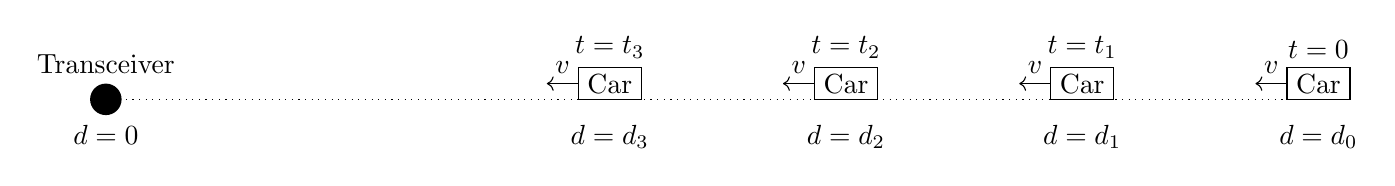
\begin{tikzpicture}

    % Draw the transceiver
    \fill[black] (0,0) circle (0.2) node[above] at (0,0.2) {Transceiver} node[below] at (0,-0.2) {$d=0$};

    % Draw the car at distance D_0
    \draw (15,0) rectangle ++(0.8,0.4) node[midway] {Car} node[above] at (15.4,0.4) {$t=0$ } node[below] at (15.4,-0.2) {$d=d_0$};
    \draw[->] (15,0.2) -- node[above] {$v$} (14.6,0.2);

    \draw (12,0) rectangle ++(0.8,0.4) node[midway] {Car} node[above] at (12.4,0.4) {$t=t_1$ } node[below] at (12.4,-0.2) {$d=d_1$};
    \draw[->] (12,0.2) -- node[above] {$v$} (11.6,0.2);

    \draw (9,0) rectangle ++(0.8,0.4) node[midway] {Car} node[above] at (9.4,0.4) {$t=t_2$ } node[below] at (9.4,-0.2) {$d=d_2$};
    \draw[->] (9,0.2) -- node[above] {$v$} (8.6,0.2);

    \draw (6,0) rectangle ++(0.8,0.4) node[midway] {Car} node[above] at (6.4,0.4) {$t=t_3$ } node[below] at (6.4,-0.2) {$d=d_3$};
    \draw[->] (6,0.2) -- node[above] {$v$} (5.6,0.2);

    \draw[dotted] (0,0) -- (15,0);

\end{tikzpicture}




    \label{fig: 1}
    \caption{}
\end{figure}

From $X\brak{j \omega}$ , we can have $x\brak{t}$ as
\begin{align}
x\brak{t} =& \dfrac{1}{2\pi} \int_{-\infty }^{\infty} X\brak{j \omega} e^{j \omega \: t} d\omega
\end{align}
For $t=0$ ,
\begin{align}
x\brak{0} =& \dfrac{1}{2\pi} \int_{-\infty }^{\infty} X\brak{j \omega} d\omega
\end{align}
On comparing , we get $A = 10$ and $ \tau = 1$,
\begin{align}
10 rect \brak{t} \longleftrightarrow 10  sinc\brak{f} 
\end{align}
\begin{figure}[ht]
	\centering
    \begin{figure}[!h]
    \centering
    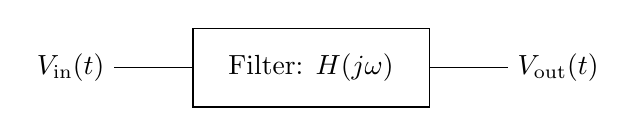
\begin{tikzpicture}
    % Draw the filter rectangle
    \draw (0,0) rectangle (3,1) node[midway] {Filter: $H(j\omega)$};
    
    % Draw the input and output labels
    \draw (-1,0.5) node[left] {$V_{\text{in}}(t)$} -- (0,0.5);
    \draw (3,0.5) -- (4,0.5) node[right] {$V_{\text{out}}(t)$};
\end{tikzpicture}
    \caption{Filter Equivalent of Circuit}
    \label{fig:2_gate.22.ee.31}
\end{figure}
    \label{fig: 2}
    \caption{}
\end{figure}
\begin{align}
10 rect \brak{t-\dfrac{1}{2}} \longleftrightarrow 10e^{-j2\pi f \times \dfrac{1}{2}}sinc \brak{f}
\end{align}
\begin{figure}[ht]
	\centering
    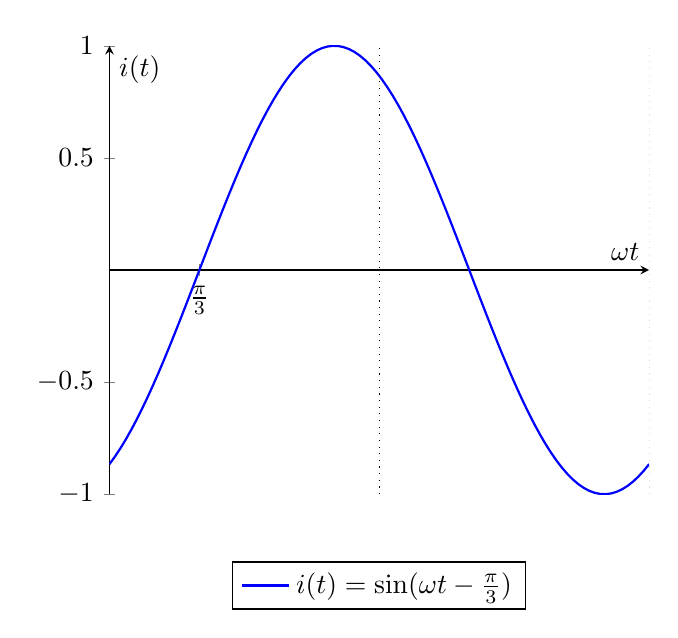
\begin{tikzpicture}

% Adjust the domain and samples according to your preference
\begin{axis}[
    xlabel={$\omega t$},
    ylabel={$i(t)$},
    domain=0:2*pi,
    samples=100,
    axis lines=middle,
    xtick={pi/3}, % Set x-axis tick at pi/3
    xticklabels={$\frac{\pi}{3}$}, % Label for the tick
    ytick={}, % Remove y-axis ticks
    legend style={at={(0.5,-0.15)},anchor=north},
]

% Plot the function
\addplot[blue,thick] {sin(deg(x - pi/3))};
\addlegendentry{$i(t) = \sin(\omega t - \frac{\pi}{3})$}

% Dotted vertical lines at x=pi and x=2pi
\draw[dotted] (axis cs:pi, \pgfkeysvalueof{/pgfplots/ymin}) -- (axis cs:pi, \pgfkeysvalueof{/pgfplots/ymax});
\draw[dotted] (axis cs:2*pi, \pgfkeysvalueof{/pgfplots/ymin}) -- (axis cs:2*pi, \pgfkeysvalueof{/pgfplots/ymax});

\end{axis}

\end{tikzpicture}

    \label{fig: 3}
    \caption{}
\end{figure}

From the above figure, $x\brak{0}$ is 10.\\
Hence, the correct option is \brak{C}.
\end{document}
\item Consider the sequence $ x_n = 0.5x_{n-1} + 1 , n = 1,2,...$ with $x_0 = 0$ Then $ \lim_{n \to \infty} x_n$ is :
\begin{enumerate}
\item[A]0
\item[B]1
\item[C]2
\item[D]$\infty$
\end{enumerate}
\hfill {GATE 2021 IN}\\
\solution
\iffalse
\let\negmedspace\undefined
\let\negthickspace\undefined
\documentclass[journal,12pt,onecolumn]{IEEEtran}
\usepackage{cite}
\usepackage{amsmath,amssymb,amsfonts,amsthm}

\usepackage{graphicx}
\usepackage{textcomp}
\usepackage{xcolor}
\usepackage{txfonts}
\usepackage{listings}
\usepackage{enumitem}
\usepackage{mathtools}
\usepackage{gensymb}
\usepackage[breaklinks=true]{hyperref}
\usepackage{tkz-euclide} % loads  TikZ and tkz-base
\usepackage{listings}
\usepackage{gvv}
\usepackage{booktabs}

%
%\usepackage{setspace}
%\usepackage{gensymb}
%\doublespacing
%\singlespacing

%\usepackage{graphicx}
%\usepackage{amssymb}
%\usepackage{relsize}
%\usepackage[cmex10]{amsmath}
%\usepackage{amsthm}
%\interdisplaylinepenalty=2500
%\savesymbol{iint}
%\usepackage{txfonts}
%\restoresymbol{TXF}{iint}
%\usepackage{wasysym}
%\usepackage{amsthm}
%\usepackage{iithtlc}
%\usepackage{mathrsfs}
%\usepackage{txfonts}
%\usepackage{stfloats}
%\usepackage{bm}
%\usepackage{cite}
%\usepackage{cases}
%\usepackage{subfig}
%\usepackage{xtab}
%\usepackage{longtable}
%\usepackage{multirow}

%\usepackage{algpseudocode}
%\usepackage{enumitem}
%\usepackage{mathtools}
%\usepackage{tikz}
%\usepackage{circuitikz}
%\usepackage{verbatim}
%\usepackage{tfrupee}
%\usepackage{stmaryrd}
%\usetkzobj{all}
%    \usepackage{color}                                            %%
%    \usepackage{array}                                            %%
%    \usepackage{longtable}                                        %%
%    \usepackage{calc}                                             %%
%    \usepackage{multirow}                                         %%
%    \usepackage{hhline}                                           %%
%    \usepackage{ifthen}                                           %%
  %optionally (for landscape tables embedded in another document): %%
%    \usepackage{lscape}     
%\usepackage{multicol}
%\usepackage{chngcntr}
%\usepackage{enumerate}

%\usepackage{wasysym}
%\documentclass[conference]{IEEEtran}
%\IEEEoverridecommandlockouts
% The preceding line is only needed to identify funding in the first footnote. If that is unneeded, please comment it out.

\newtheorem{theorem}{Theorem}[section]
\newtheorem{problem}{Problem}
\newtheorem{proposition}{Proposition}[section]
\newtheorem{lemma}{Lemma}[section]
\newtheorem{corollary}[theorem]{Corollary}
\newtheorem{example}{Example}[section]
\newtheorem{definition}[problem]{Definition}
%\newtheorem{thm}{Theorem}[section] 
%\newtheorem{defn}[thm]{Definition}
%\newtheorem{algorithm}{Algorithm}[section]
%\newtheorem{cor}{Corollary}
\newcommand{\BEQA}{\begin{eqnarray}}
\newcommand{\EEQA}{\end{eqnarray}}
\newcommand{\define}{\stackrel{\triangle}{=}}
\theoremstyle{remark}
\newtheorem{rem}{Remark}

%\bibliographystyle{ieeetr}
\begin{document}
%

\bibliographystyle{IEEEtran}


\vspace{3cm}

\title{
%	\logo{
Gate 2021 Assignment 

\large{EE:1205 Signals and Systems}

Indian Institute of Technology, Hyderabad
%	}
}
\author{Abhey Garg

EE23BTECH11202
}	


% make the title area
\maketitle



%\tableofcontents


\renewcommand{\thefigure}{\theenumi}
\renewcommand{\thetable}{\theenumi}
%\renewcommand{\theequation}{\theenumi}

\section{Question IN 02}
Consider the sequence $ x_n = 0.5x_{n-1} + 1 , n = 1,2,...$ with $x_0 = 0$ Then $ \lim_{n \to \infty} x_n$ is :
\begin{enumerate}
\item[A]0
\item[B]1
\item[C]2
\item[D]$\infty$
\end{enumerate}
\section{Solution}
\fi
\begin{align}
x_n = 0.5 x_{n-1} + 1
\end{align}
Taking Z-transform:
\begin{align}
X(z) = 0.5 z^{-1} X(z) + \frac{1}{1-z^{-1}} \\
X(z)[1-0.5z^{-1}] = \frac{1}{1-z^{-1}} \\
X(z) = \frac{1}{(1-z^{-1})(1-0.5z^{-1})}\\
X(z) = \frac{A}{1-z^{-1}} + \frac{B}{1-0.5z^{-1}}\\
A+B = 1 \\
A = -2B \\
A = 2 \\
B = -1 \\
X(z) = \frac{2}{1-z^{-1}} + \frac{-1}{1-0.5z^{-1}}\\
\end{align}
Taking inverse Z-transform:
\begin{align}
x(n) = 2 u(n) + (-1)(0.5^n)u(n)\\
\lim_{n \to \infty} x(n) = 2
\end{align}

%\end{document}

\end{enumerate}

 \section{2021}
 
\backmatter
\appendix
\chapter{Fourier transform}
\chapter{Contour Integration}
\iffalse
\chapter{ Convolution}
\chapter{ Z-transform}
\fi
\latexprintindex
\end{document}

 
